% ============================================================
%  Modeling Radioresistance and Radiotropic Fitness
%  Hunter Kinder & Brett Faulkner
%  NOTE: the file name still reads modeling_radiotrophic_fitness.*; the rename
%  is deferred to a separate commit so this revision's diff stays readable.
%  See docs/preprint_revision_plan.md.
%  Preprint — bioRxiv Systems Biology — April 2026
% ============================================================
\documentclass[11pt]{article}

% --- Geometry -----------------------------------------------
\usepackage[top=1in,bottom=1in,left=1.1in,right=1.1in]{geometry}

% --- Encoding & fonts ----------------------------------------
\usepackage[T1]{fontenc}
\usepackage[utf8]{inputenc}
\usepackage{lmodern}
\usepackage{microtype}

% --- Math ---------------------------------------------------
\usepackage{amsmath,amssymb,amsthm}
\usepackage{bm}

% --- Tables -------------------------------------------------
\usepackage{booktabs}
\usepackage{array}
\usepackage{tabularx}
\usepackage{longtable}
\usepackage{rotating}
\usepackage{pdflscape}

% --- Graphics & colour ----------------------------------------
\usepackage{graphicx}
\graphicspath{{figures/}}
\usepackage{xcolor}
\definecolor{linkblue}{RGB}{0,70,150}

% --- Hyperref ------------------------------------------------
\usepackage[colorlinks=true,
            linkcolor=linkblue,
            citecolor=linkblue,
            urlcolor=linkblue,
            pdftitle={Modeling Radioresistance and Radiotropic Fitness},
            pdfauthor={Hunter Kinder, Brett Faulkner}]{hyperref}

% --- Layout ---------------------------------------------------
\usepackage{parskip}
\setlength{\parskip}{6pt}
\usepackage{setspace}
\setstretch{1.15}
\usepackage{titlesec}
\titleformat{\section}{\large\bfseries}{\thesection.}{0.5em}{}
\titleformat{\subsection}{\normalsize\bfseries}{\thesubsection}{0.5em}{}
\titlespacing{\section}{0pt}{14pt}{6pt}
\titlespacing{\subsection}{0pt}{10pt}{4pt}

% --- Floats & captions ----------------------------------------
\usepackage{caption}
\captionsetup{font=small,labelfont=bf}

% (no datetime2 in basic install)

% ============================================================
\begin{document}

% ---- Title block --------------------------------------------
\begin{center}
  {\LARGE\bfseries Modeling Radioresistance and Radiotropic Fitness}\\[10pt]
  {\large\bfseries Spatiotemporal Dynamics of Microbial Communities\\
   Under Ionizing Radiation Stress}\\[14pt]
  {\normalsize
    \textbf{Hunter Kinder}, B.A., M.A.T.L. --- Independent Researcher, Missouri, USA\\[2pt]
    \textbf{Brett Faulkner}, B.Sc, BioPhys --- Independent Researcher\\[10pt]
  }
  {\small
    \textit{Preprint --- submitted to bioRxiv (Systems Biology)}\\
    \textit{Version 1.0 --- April 2026}
  }
\end{center}
\vspace{4pt}
\noindent\rule{\linewidth}{0.5pt}
\vspace{2pt}

% ---- Abstract ------------------------------------------------
\begin{abstract}
\noindent
This work presents a mathematical framework for the spatial and adaptive dynamics of microbial
communities exposed to gamma radiation. The developed model integrates Langevin dynamics with
reaction-diffusion equations to simulate the spatial motility and nonlinear interactions of
melanized fungi, radioresistant extremophiles, and radiosensitive species. In this framework,
radiation gradients and chemical factors, such as melanin synthesis, are introduced as modifiable
parameters to analyze their influence on biofilm organisation. Numerical simulations of seven
interacting species---including \textit{Cryptococcus neoformans}, \textit{Deinococcus radiodurans},
\textit{Cladosporium sphaerospermum}, \textit{Bacillus subtilis}, \textit{Aspergillus niger},
\textit{Shewanella oneidensis}, and \textit{Ochrobactrum intermedium} AM7---produce radial
structure on the Cellular Potts lattice, which we report with the qualification it needs. The
modelled field is maximal on the cylinder axis and decays outward, so the core is the high-dose
region; the melanized fungi end the run at \emph{larger} radius than \textit{B.~subtilis}, which is
the direction opposite to the one their negative $\beta_{s,\mathrm{ion}}$ implements. With six
parcels per species on a single seed the separation is not yet distinguishable from the uniform-disk
initial condition (Section~\ref{sec:cpm_results}), and no multi-seed run against that null has been
performed.

We are explicit about which radiation phenotype this is. What the model expresses is
\emph{radiotropism}: a directional spatial preference in a dose gradient, set by the sign of the
per-species coefficient $\beta_{s,\mathrm{ion}}$. It is not \emph{radiotrophy} (ionizing radiation
measurably enhancing growth or metabolism), because the simulations create no biomass, and it is
not \emph{radioresistance} (elevated survival), because they impose no death; both are structurally
absent rather than weakly supported. The published $D_{10}$ radioresistance evidence that anchors
the per-species magnitudes in Table~\ref{tab:params} is therefore radioresistance evidence spent on
a tropism coefficient, which we declare here rather than leave implicit in a sign convention.
Radiotrophy is additionally not established for any of the seven species modelled
(Section~\ref{sec:radiotrophy_status}). Within those limits the framework offers a route to
reasoning about spatial self-organisation of microbial consortia under heterogeneous radiation
fields, with applications to nuclear bioremediation.
\end{abstract}
\noindent\rule{\linewidth}{0.5pt}

% ---- 1. Introduction -----------------------------------------
\section{Introduction}

Microbial communities possess an extraordinary ability to adapt and survive under extreme
environmental stressors, such as elevated radiation levels. Within such communities, melanized
fungi and other extremophilic microorganisms have evolved specialized mechanisms that allow them
to persist in high-radiation environments. This study aims to develop a comprehensive mathematical
framework that captures the complex interplay between these organisms' nonlinear interactions,
radiation sensitivities, and chemotactic behaviors within biofilm communities. By leveraging a
combined approach that integrates Langevin dynamics, reaction-diffusion modeling, and a
Hamiltonian-based formulation, we simulate and explore the spatiotemporal evolution of these
communities under radiation stress and other external influences.

The practical motivation for this work lies in nuclear bioremediation. Contaminated sites such
as the Chernobyl Exclusion Zone and the Hanford Nuclear Reservation host complex microbial
communities in which melanized and radioresistant species coexist with metal-reducing bacteria
capable of immobilizing radionuclides. Mathematical models that predict community dynamics under
spatially heterogeneous radiation fields are essential for designing and optimizing bioremediation
strategies. The framework developed here provides the theoretical foundation for such predictions.

Five phenomena travel under one loose vocabulary and they are not interchangeable: \emph{radiotropic}
(directional growth or redistribution relative to a source), \emph{radiotrophic} (radiation
measurably enhancing growth or metabolism), \emph{radioresistant} (elevated survival after
exposure), \emph{melanized radioprotective} (melanin measurably altering damage, survival or
shielding), and \emph{radiation-responsive} (any molecular, morphological or material change after
exposure). A survival curve cannot calibrate a directional term, and a transcriptome cannot set a
material density. Throughout this paper we use each word only for the endpoint it names. The model
presented here expresses the first of the five, and the paper's title says so.

% ---- 2. Related Work -----------------------------------------
\section{Related Work}

\subsection{Melanized Fungi, Radioresistance, and the Contested Radiotrophy Claim}

The observation that melanized fungi colonise high-radiation environments prompted a proposal that
melanin transduces ionizing radiation into metabolically usable energy. That proposal remains
contested, and this subsection reports it as a live dispute rather than as settled background.
Zhdanova et al.\ \cite{zhdanova2000}
first documented the prevalence of darkly pigmented fungi within the damaged reactor at the
Chernobyl Nuclear Power Plant, noting that species such as \textit{Cladosporium sphaerospermum}
dominated the mycobiota of the most contaminated structures. Subsequent work by Dadachova et
al.\ \cite{dadachova2007} demonstrated that ionizing radiation alters the electronic properties of
melanin, enhancing electron-transfer activity in melanized cells of \textit{Cryptococcus neoformans}
and \textit{Wangiella dermatitidis}. Melanized cells exposed to radiation levels approximately 500
times above background grew significantly faster, accumulated more biomass, and incorporated
three-fold more ${}^{14}$C-acetate than non-irradiated melanized cells or irradiated albino
mutants. Dadachova and Casadevall \cite{dadachova2008} subsequently proposed the term
``radiosynthesis'' to describe this phenomenon, drawing an analogy to photosynthesis in which
melanin serves a role loosely comparable to chlorophyll. Three features of the founding experiment
are usually omitted when it is cited and are reported here: the cell arm was a $^{188}$Re beta
field at 0.05~mGy~h$^{-1}$ rather than a photon field; the growth effects are single-digit
percentages in dry weight; and non-irradiated non-melanized cells grew better than non-irradiated
melanized cells in the same experiment, so the melanized/albino contrast carries a baseline
asymmetry present before any radiation was applied \cite{audit2026}.

Shunk et al.\ \cite{shunk2022} cultivated \textit{C.\ sphaerospermum} aboard the International
Space Station for 26 days, reporting a growth ratio of $1.21 \pm 0.37$-fold against the ground
control and lower counts beneath the fungal biomass. Neither result is a demonstration of
radiotrophy and neither should be quoted without its interval: the stated ratio does not exclude
unity, the attenuation comparison reached $p = 0.069$ on a single dish with one sensor pair, no
dosimetric data were obtained (the sensors were PIN photodiodes), melanin was never measured, and
the words ``radiotrophic'' and ``radiation-shield'' were struck from the title between preprint and
publication \cite{audit2026}. The commonly circulated ``$2.17 \pm 0.25\%$'' attenuation figure
appears in no version of that work.

The radiation resistance of \textit{Deinococcus radiodurans} operates through fundamentally
different mechanisms. Rather than harnessing radiation for metabolic benefit, \textit{D.\
radiodurans} survives doses exceeding 12~kGy through a combination of efficient DNA
double-strand break repair via extended synthesis-dependent strand annealing (ESDSA), multiple
genome copies enabling homologous recombination, and a potent manganese-based antioxidant system
that protects proteins from oxidative damage \cite{slade2011,daly2009}. Daly et al.\
\cite{daly2010} showed that small-molecule Mn$^{2+}$-metabolite complexes specifically protect
the proteome against radiation-induced carbonylation, establishing that protein protection, rather
than DNA repair capacity alone, governs extreme radioresistance. This is the best-evidenced
radiation phenotype in the set of species modelled here, and it is a survival phenotype.

\textit{Aspergillus niger} is melanized, and an earlier draft of this work asserted that its
melanin confers substantial radioprotection. The isogenic test contradicts that assertion and it
is withdrawn. Cortes\~{a}o et al.\ \cite{cortesao2020} compared \textit{A.\ niger} N402 with its
pigmentation-deficient $\Delta fwnA$ mutant MA93.1 and found LD$_{90}$ values of 366 against
353~Gy (X-ray), 506 against 567~Gy (helium ions) and 112 against 112~Gy (iron ions) --- one pair
running in the wrong direction and none of the three separable. What carried resistance in that
dataset was DNA repair: the NHEJ mutant collapsed to LD$_{90}$ 57 / 55 / 50~Gy. The same null has
been reported three times independently in \textit{Exophiala dermatitidis} wild type against its
non-melanized \textit{pks1} mutant across gamma, alpha, proton and deuteron exposure
\cite{audit2026}.

\subsection{Mathematical Models of Biofilm Communities}

The mathematical modeling of biofilm communities has a rich history beginning with the
foundational one-dimensional multispecies model of Wanner and Gujer \cite{wanner1986}, which
coupled reaction-diffusion equations for substrate transport with biomass conservation laws to
predict biofilm thickness and spatial species distributions. Xavier et al.\ \cite{xavier2005}
extended this framework to multiple spatial dimensions, providing a deterministic continuum
approach to heterogeneous biofilm development. Individual-based modeling approaches, exemplified
by the iDynoMiCS platform of Lardon et al.\ \cite{lardon2011}, complement continuum models by
resolving cell-level stochastic interactions. Cross-diffusion biofilm models have been analyzed
by Sonner et al.\ \cite{sonner2015}, who established mathematical properties of volume-filling
multispecies systems that exhibit porous-medium-type degeneracy. Our PSDE framework extends
these precedents by incorporating radiation-dependent fitness terms and phase-locking dynamics
that couple species interactions to external radiation fields, moving beyond the
substrate-limited growth paradigms that dominate existing biofilm models.

\subsection{Hamiltonian and Stochastic Approaches in Theoretical Ecology}

The application of Hamiltonian mechanics to ecological systems remains comparatively
underexplored, despite the natural conservation laws that govern energy flow in ecosystems.
Symplectic integration methods, which preserve the geometric structure of Hamiltonian flows,
have been advocated for ecological modeling by Diele et al.\ \cite{diele2015} to ensure that
numerical solutions maintain essential qualitative dynamics. The Kuramoto model of coupled phase
oscillators \cite{kuramoto1984} provides a well-established framework for synchronization
phenomena in biological systems, from neural networks to circadian rhythms. Aceb\'r\'on et al.\
\cite{acebron2005} reviewed the model as a paradigm for synchronization, noting its
generalization to systems with time delays, frequency-weighted coupling, and heterogeneous
interaction topologies. Our phase-locking kernel $\Gamma_s(t,\mathbf{x})$ draws directly on
this tradition, extending it to multispecies microbial communities where species-level
oscillatory dynamics in growth and resource acquisition couple through shared radiation and
nutrient fields. The use of Langevin stochastic dynamics to describe microbial population
fluctuations follows naturally from the Fokker-Planck formalism and has been applied to
competing microbial populations in chemostat systems \cite{campillo2017}, where stochastic
differential equations revealed long-term competitive outcomes differing from deterministic
predictions.

\subsection{Bioremediation Context}

The practical motivation for modeling these communities lies in nuclear bioremediation.
\textit{Shewanella oneidensis} MR-1 is a model dissimilatory metal-reducing bacterium capable
of reducing soluble U(VI) to insoluble U(IV) via extracellular electron transfer through
c-type cytochromes \cite{heidelberg2002,veeramani2011}. \textit{Ochrobactrum intermedium} AM7,
isolated from soil near the Kakrapar Atomic Power Station in India, tolerates high concentrations
of thorium and produces exopolysaccharides (EPS) that complex with Th(IV), offering a pathway
toward bioremediation of actinide-contaminated environments \cite{shukla2020}. The combination
of melanized fungi that persist in the high-dose zone with metal-reducing bacteria that
immobilize radionuclides suggests the possibility of engineered biofilm consortia for in situ
remediation. The fitness landscape framework introduced by Wright \cite{wright1932} and
formalized through the NK model of Kauffman \cite{kauffman1989} provides a conceptual foundation
for understanding how epistatic interactions among species traits shape adaptation under
radiation stress, a perspective that our Hamiltonian kNN decision tree operationalizes
quantitatively.

\subsection{Radiotrophy Is Not Established for Any Species Modelled Here}
\label{sec:radiotrophy_status}

Because this paper models seven named species, we audited the public evidence for the radiation
phenotype of each rather than importing the labels on reputation. The audit
\cite{audit2026} searched eleven data repositories at the API level (Dryad, Zenodo, Figshare, EBI
BioImage Archive, BioStudies, IDR, EMPIAR, NASA OSDR, heiDATA, DepositOnce, MINDS@UW), the NCBI
sequence and functional-genomics archives, and Europe PMC, and assigned every phenotype label from
the endpoint actually measured. Its verdict on the phenotype in this paper's former title is
\texttt{TARGETED\_LAB\_EXPERIMENT\_REQUIRED}, and its finding is unambiguous:

\begin{quote}
Radiotrophy is not established for any of the seven species modelled.
\end{quote}

The claim rests on a single 2007 paper covering two of the seven, and against it stand a
same-species report of no substantial melanin protection under gamma, a same-species negative
melanin-pathway result at 1 and 3~kGy, a same-genus null growth result under a TLD-anchored
$^{137}$Cs field, an isogenic null in \textit{A.\ niger} across three ionizing modalities
(Section~2.1), and a formal energy-budget critique holding that the deposited energy is
insufficient and the media carbon sufficient to account for the observed growth
\cite{walberg2015}. ``Not demonstrated'' is not ``disproved'', and we state it as the former.

Radioresistance, by contrast, is well evidenced for several of the seven, and the
$D_{10}$ values in Table~\ref{tab:params} are real measurements. Radiotropism has its own
candidate --- Zhdanova et al.'s 2004 report of directed hyphal growth toward a $^{109}$Cd source,
with \textit{C.\ sphaerospermum} 3176 among the responders --- and that record is blocked twice
over: whether its dose gradient was measured or calculated is unverified, and directed hyphal
elongation has no representation in a model whose agents are isotropic biomass parcels with no
elongation or connectivity term. Three further audit verdicts bound what public data can do for
this model at all: the CPM spatial machinery can be exercised but not calibrated on public data
(\texttt{PUBLIC\_DATA\_CAN\_VALIDATE\_PIPELINE\_ONLY}); no public source pairs a calibrated
hydrated volume with wet mass, dry mass and matched blanks
(\texttt{TARGET\_WET\_BULK\_MEASUREMENT\_REQUIRED}); and no dataset anywhere pairs an exact
modelled species with both a calibrated 3-D biomass field and a characterised radiation exposure
(\texttt{PUBLIC\_COMPONENTS\_FOUND\_BUT\_NOT\_PAIRED}). Every parameter in Table~\ref{tab:params}
is therefore a literature-anchored prior, and a literature prior is not a calibration.

% ---- 3. Mathematical Framework --------------------------------
\section{Mathematical Framework}

\subsection{Symbols and Notation}

\begin{table}[h!]
\centering
\small
\caption{Summary of principal mathematical symbols.}
\label{tab:notation}
\begin{tabular}{@{}lp{0.72\linewidth}@{}}
\toprule
\textbf{Symbol} & \textbf{Description} \\
\midrule
$F_s(t,\mathbf{x})$ & Fitness function of species $s$, evolving over time $t$ and space $\mathbf{x}$ \\
$H(p,q)$            & Hamiltonian function defining total system energy \\
$p,\,q$             & Phase-space variables (generalised momentum and position) \\
$\eta_s(t,\mathbf{x}) = \sigma_s\xi(t,\mathbf{x})$ & Stochastic noise: $\sigma_s$ intensity; $\xi$ spatiotemporal white noise \\
$D_s$               & Species-specific passive diffusion coefficient \\
$\mu_s$             & Species-specific directed-motility (chemotaxis) coefficient \\
$P_{sj}(t)$         & Permutation matrix describing species-$s$ to species-$j$ transitions \\
$I_\gamma(t,\mathbf{x})$ & Ionizing (gamma) radiation field \\
$N(t,\mathbf{x})$   & Non-ionizing (UV) radiation field \\
$k_B$               & Boltzmann constant \\
$S[q(t)]$           & Action functional for species trajectories \\
$\nabla$            & Spatial gradient operator \\
$\Gamma_s(t,\mathbf{x})$ & Phase-locked kernel for species $s$ \\
$\beta_{s,\mathrm{ion}}$ & Ionizing radiation coefficient. In the PSDE (Eq.~\ref{eq:psde}) a fitness-loss rate; in the CPM (Section~\ref{sec:methods}) a \emph{tropism} coefficient whose sign sets the direction of drift along the dose gradient. Magnitudes anchored to published $D_{10}$ radioresistance data (Table~\ref{tab:params}) \\
$\alpha_{s,\mathrm{nir}}$ & Non-ionizing radiation coupling coefficient \\
$\theta_s$          & Adaptive phase-locking coefficient \\
$\gamma_s$          & Gamma-radiation coupling coefficient in the adaptive-feedback term (Eq.~\ref{eq:adaptive}) \\
$\Delta_s$          & Phase-locking synchronization deviation \\
\bottomrule
\end{tabular}
\end{table}

\subsection{Partial Stochastic Differential Equation (PSDE) for Species Fitness}

The fitness of each species $s$ is governed by the following PSDE:
\begin{align}
\partial_t F_s
  &= \nabla\!\cdot(D_s\nabla F_s)
   - \nabla\!\cdot\!\left(\mu_s\sum_{j=1}^n P_{sj}(t)\,F_j\right)
   + R_s
   + \sigma_s\xi(t,\mathbf{x}) \notag \\
  &\quad
   - \beta_{s,\mathrm{ion}}\,I_\gamma F_s
   + \gamma_s\Delta_s
   - \alpha_{s,\mathrm{nir}}\,N F_s
   + \theta_s H_s
   + C_s
  \label{eq:psde}
\end{align}

\noindent where $F_s \equiv F_s(t,\mathbf{x})$, $I_\gamma \equiv I_\gamma(t,\mathbf{x})$, and
$N \equiv N(t,\mathbf{x})$.  The nine terms encode:
\begin{itemize}\setlength\itemsep{2pt}
  \item \textbf{Diffusion}: passive spatial spreading at rate $D_s$.
  \item \textbf{Directed motility}: chemotaxis and radiation-gradient-directed movement
        controlled by $\mu_s$ and the transition matrix $P_{sj}$.
  \item \textbf{Deterministic reaction}: $R_s(t,\mathbf{x})$, nutrient-dependent growth
        (see Section~\ref{sec:nutrient}).
  \item \textbf{Stochastic noise}: $\sigma_s\xi(t,\mathbf{x})$, spatiotemporal white noise
        scaled by species noise intensity $\sigma_s$.
  \item \textbf{Ionising damage}: $-\beta_{s,\mathrm{ion}}\,I_\gamma(t,\mathbf{x})\,F_s$,
        radiation-induced fitness reduction.
  \item \textbf{Phase-locking adjustment}: $\gamma_s\Delta_s$, adaptive synchronisation gain
        from melanin-mediated energy transduction.
  \item \textbf{Non-ionising effect}: $-\alpha_{s,\mathrm{nir}}\,N(t,\mathbf{x})\,F_s$,
        UV/heat-driven fitness coupling.
  \item \textbf{Hamiltonian interaction}: $\theta_s H_s(t,\mathbf{x})$, energy-conserving
        inter-species force from the Hamiltonian (Section~\ref{sec:hamiltonian}).
  \item \textbf{External forcing}: $C_s(t,\mathbf{x})$, environmental control inputs.
\end{itemize}

\paragraph{This subsection is specification, not method.}
No program in this work integrates Eq.~\ref{eq:psde}. There is no fitness field $F_s$ in any
source file: a case-insensitive search for it across every \texttt{.jl} and \texttt{.R} file
returns only the manuscript title in header comments. What the three R codes advance is a set of
particle positions under overdamped first-order Euler steps, and the CPM advances a lattice
configuration by Metropolis acceptance --- neither is a discretisation of a field equation in
$F_s$.

Four of the nine terms are additionally unrepresentable rather than merely unimplemented. The
deterministic reaction $R_s$ is nutrient-dependent \emph{growth}, and the CPM has none:
\texttt{state.nutrient} is written each step but never read by \texttt{compute\_delta\_H}, and
\texttt{divide\_cell!} has no trigger. The phase-locking adjustment $\gamma_s\Delta_s$ depends on
the $H_{\mathrm{kNN}}$ machinery of Section~3.8, which is specified and unexercised. The
non-ionising term $\alpha_{s,\mathrm{nir}}N$ and the external forcing $C_s$ have no counterpart in
any state variable. Only diffusion, directed motility, noise and the ionising term have anything
in the implemented models that corresponds to them, and even those correspond by analogy rather
than by discretisation --- the CPM's radiation term is an acceptance bias, not a fitness sink.

Eq.~\ref{eq:psde} is therefore the framework this work proposes, and the simulations reported in
Section~\ref{sec:results} are separate, simpler models that share its vocabulary. Presenting the
two as one system would be the central error this manuscript exists to avoid.

\subsection{Hamiltonian Framework}
\label{sec:hamiltonian}

The total Hamiltonian for the multi-species biofilm is:
\begin{equation}
\label{eq:hamiltonian}
H = \sum_{i=1}^{N}\!\left[\frac{1}{2}\,\rho_i\,v_i^2 + U_i(\mathbf{x}_i)\right]
  + \sum_{i\neq j} V_{ij}(r_{ij})
  + \sum_{k=1}^{K} W_k(t,\mathbf{x})
\end{equation}

\noindent where $\rho_i$ is the effective biomass density of species $i$ [cells\,$\mu$m$^{-3}$
$\times$ effective mass analog], $U_i(\mathbf{x}_i)$ is the potential energy in the nutrient
concentration field, $V_{ij}(r_{ij})$ is the pairwise interaction energy, and $W_k(t,\mathbf{x})$
captures external energy contributions from radiation exposure and stochastic effects. For
mutualistic interactions:
\begin{equation}
  V_{ij}^{\mathrm{mutual}}(r_{ij}) = -\gamma\,\exp\!\left(-\frac{r_{ij}^2}{\sigma^2}\right)
\end{equation}

\subsection{Symplectic Integration}

Symplectic integrators preserve the geometric structure of the Hamiltonian flow, ensuring that
energy and momentum do not drift over extended simulation windows. Phase-space trajectories
evolve via the phase-locked canonical equations:
\begin{equation}
\label{eq:canonical}
\frac{dq}{dt} = \frac{\partial H}{\partial p} - \Gamma_s(t,\mathbf{x})\,F_s(t,\mathbf{x}),
\qquad
\frac{dp}{dt} = -\frac{\partial H}{\partial q} + \Gamma_s(t,\mathbf{x})\,F_s(t,\mathbf{x})
\end{equation}

The leapfrog/Verlet scheme is the intended numerical treatment: (1) evaluate $H_s$ from the
current state; (2) adjust the phase-locking deviation $\Delta_s$; (3) advance via a symplectic step
\cite{hairer2006}.

\paragraph{This subsection is specification, not method.}
No program in this work performs symplectic integration. Eq.~\ref{eq:hamiltonian} carries a kinetic
term, but no simulation reported here holds a velocity or momentum state: the R models advance
positions under overdamped first-order Euler steps and the CPM is a Metropolis Markov chain, which
has no trajectory whose symplectic form could be preserved. Implementing it is listed in
Section~\ref{sec:limitations}.

\subsection{Radiation Field Models}

\paragraph{Ionizing radiation (gamma decay).}
\begin{equation}
\label{eq:gamma_field}
I_\gamma(t,\mathbf{x}) = I_0\,\exp(-\kappa\,\|\mathbf{x}\|)
\end{equation}
where $I_0$ is the initial intensity at the source and $\kappa$ is the attenuation coefficient
scaled by local biofilm density.

\paragraph{Non-ionizing radiation (UV oscillatory field).}
\begin{equation}
\label{eq:uv_field}
N(t,\mathbf{x}) = N_{\mathrm{UV}}\cos(\omega t)
\end{equation}

\subsection{Melanin Reaction-Diffusion}

The spatial production and diffusion of melanin by the melanized fungi is modelled as:
\begin{equation}
\label{eq:melanin}
\frac{\partial M}{\partial t} = D_M\,\nabla^2 M + \alpha_M\cdot n_{\mathrm{RF}}(\mathbf{x},t)\cdot I_\gamma(t,\mathbf{x})
\end{equation}
where $D_M$ is the melanin diffusion coefficient [$\mu$m$^2$\,s$^{-1}$], $\alpha_M$ is the
radiation-driven production rate [$\mu$g cell$^{-1}$ Gy$^{-1}$], and $n_{\mathrm{RF}}$ is the
local melanized-fungal cell density [cells\,$\mu$m$^{-3}$]. Each term carries units of
[$\mu$g\,$\mu$m$^{-3}$\,s$^{-1}$].

The sign of $\alpha_M$ is a modelling assumption and the evidence runs against it. A same-species,
same-modality measurement in \textit{C.\ neoformans} found the melanin-synthesis genes \textit{LAC1}
and \textit{LAC2} \emph{down}-regulated after 1 and 3~kGy of gamma, and a two-species pigmentation
assay found pigmentation increased under UV but decreased under gamma, both at $P < 0.001$
\cite{audit2026}. Equation~\ref{eq:melanin} as written, with $\alpha_M > 0$, therefore encodes the
opposite sign to the only same-modality data located. It is retained here so that the assumption is
visible and testable, not because it is supported.

\subsection{Nutrient Uptake with Adaptive Feedback}
\label{sec:nutrient}

\begin{equation}
\label{eq:nutrient}
R_s(t,\mathbf{x}) = \alpha_s\,C_s(t,\mathbf{x})\!\left(1 - \frac{F_s(t,\mathbf{x})}{K_s}\right)
  + A_s(t)\,C_s(t,\mathbf{x})
\end{equation}
\begin{equation}
\label{eq:adaptive}
A_s(t) = \gamma_s\,\phi_s(t) - \beta_{s,\mathrm{ion}}\,I_\gamma(t)
\end{equation}
where $\phi_s(t) = \cos(\omega_s t - \theta_s)$ is the phase-alignment function and $A_s(t)$ is
the adaptive feedback driven by phase-locking and local radiation stress.

\subsection{Hamiltonian kNN Decision Tree}

To model species transition probabilities modulated by neighbourhood phase states:
\begin{equation}
\label{eq:knn}
H_{\mathrm{kNN}} = \frac{1}{\sigma_n}\sum_{j=1}^{n} P_{sj}(t)\,F_j(t,\mathbf{x})\,\Gamma_s(t,\mathbf{x})
\end{equation}

\subsection{Radiation Damage and Resilience}

\begin{equation}
\label{eq:damage}
D_{\mathrm{rad},s}(t,\mathbf{x}) = -\beta_{s,\mathrm{rad}}\,I_\gamma(t,\mathbf{x})\,F_s(t,\mathbf{x})
\end{equation}
Species with stronger DNA repair or antioxidant protection exhibit lower $\beta_{s,\mathrm{rad}}$
values, reflecting the Mn$^{2+}$-dependent proteome protection described by Daly et al.\
\cite{daly2010}. The parameterisation additionally assigns low $\beta_{s,\mathrm{rad}}$ to the
melanized species. That is a modelling assumption and the isogenic evidence does not support it:
melanin knockouts show no survival difference under ionizing radiation in \textit{A.\ niger}
\cite{cortesao2020} or in three independent \textit{E.\ dermatitidis} studies across four
modalities \cite{audit2026}. Where melanin measurably mattered in an evolution experiment, it
reduced mutation accumulation without altering survival --- an effect on damage that must not be
generalised into a survival term.

\subsection{Biofilm Mechanical Properties}

The EPS matrix is modelled as a Finite Extensible Nonlinear Elastic (FENE) entropic spring:
\begin{equation}
\label{eq:fene}
U(r) = -\frac{1}{2}\,k\,R^2\,\ln\!\left(1 - \frac{r^2}{R^2}\right)
\end{equation}
where $k$ is the spring constant, $R$ is the maximum extensibility, and $r$ is the current
end-to-end distance.  Viscoelastic creep follows the Kelvin-Voigt model:
\begin{equation}
\label{eq:kelvinvoigt}
\sigma(t) = E\,\varepsilon(t) + \eta\,\frac{d\varepsilon}{dt}
\end{equation}
with stress relaxation time $\tau = \eta/E$ governing biofilm restructuring dynamics.

\subsection{Radiodialysis Membrane Transport}
\label{sec:radiodialysis}

To model contaminant ingress through the bioreactor membrane under radiation-driven
permeability change, we introduce a minimal three-equation system coupling mobile
contaminant transport, biosorption/bioreduction, and membrane structural damage.

\paragraph{Mobile contaminant --- cylindrical reaction-diffusion.}
The concentration $c(r,t)$ of a dissolved contaminant (e.g.\ aqueous U(VI), Cs$^+$) in the
cylindrical biofilm domain satisfies:
\begin{equation}
\frac{\partial c}{\partial t}
  = \frac{1}{r}\frac{\partial}{\partial r}\!\left(r\,D_{\mathrm{eff}}\frac{\partial c}{\partial r}\right)
  - \bigl(k_{\mathrm{ads}}X + k_{\mathrm{red}}X_{\mathrm{red}}\bigr)\,c
  + k_{\mathrm{des}}\,s
\label{eq:mobile}
\end{equation}
where $D_{\mathrm{eff}}$ is the effective diffusivity through the EPS matrix,
$k_{\mathrm{ads}}$ and $k_{\mathrm{red}}$ are the biosorption and bioreduction rate constants,
$X$ and $X_{\mathrm{red}}$ are the total and metal-reducing biomass densities, and $s(r,t)$
is the immobilised contaminant concentration (sorbed or reduced phase).
Zero-flux symmetry is imposed at $r = 0$.

\paragraph{Immobile phase --- biosorption and bioreduction.}
\begin{equation}
\frac{\partial s}{\partial t}
  = \bigl(k_{\mathrm{ads}}X + k_{\mathrm{red}}X_{\mathrm{red}}\bigr)\,c
  - \bigl(k_{\mathrm{des}} + k_{\mathrm{loss}}\bigr)\,s
\label{eq:immobile}
\end{equation}
where $k_{\mathrm{loss}}$ accounts for precipitation, co-precipitation, or export of the
immobilised fraction \cite{renslow2017}.

\paragraph{Membrane damage and radiation-driven permeability.}
Radiation progressively degrades membrane structural integrity $m(t) \in [0,1]$:
\begin{equation}
\frac{dm}{dt} = -k_{\mathrm{dam}}\,\dot{D}(R)\,m, \qquad m(0)=1
\label{eq:membrane_damage}
\end{equation}
where $\dot{D}(R)$ is the absorbed dose rate at the membrane wall ($r=R$).
The effective permeability $P_{\mathrm{eff}}$ evolves with cumulative dose
$D_{\mathrm{cum}}(t) = \dot{D}(R)\cdot t$:
\begin{equation}
P_{\mathrm{eff}}(t) = P_0\,\exp\!\bigl(\alpha_P\,D_{\mathrm{cum}}(t)\bigr)
\label{eq:peff}
\end{equation}
consistent with radiation-driven permeability enhancement observed in Nafion membranes under
ionising flux \cite{lara2023}.

\paragraph{Robin boundary condition at $r = R$.}
The membrane couples interior concentration gradient to the external reservoir $c_{\mathrm{ext}}$:
\begin{equation}
-D_{\mathrm{eff}}\left.\frac{\partial c}{\partial r}\right|_{r=R}
  = P_{\mathrm{eff}}(t)\,\bigl(c(R,t) - c_{\mathrm{ext}}\bigr)
\label{eq:robin}
\end{equation}
This is analogous to Donnan dialysis through a charged membrane \cite{aydogan2022,fox2009},
with the critical distinction that $P_{\mathrm{eff}}$ is not a fixed material property but an
evolving field driven by cumulative radiation exposure --- a self-regulating mechanism in which
the radiation that sustains the biofilm simultaneously widens the pathway for contaminant
uptake.

% ---- 4. Parameter Estimation ----------------------------------
\section{Parameter Estimation}

Biologically justified parameter ranges for the six primary modelled species, derived from
published experimental data, are given in Table~\ref{tab:params}. Three declarations govern how
that table should be read.

\emph{These are priors, not calibrations.} No value in Table~\ref{tab:params} was fitted to data
from this system, and no optimisation was performed (Section~\ref{sec:methods}). A literature prior
is not a calibration and must not be reported as one.

\emph{The $\beta_{s,\mathrm{ion}}$ column spends radioresistance evidence on a tropism
coefficient.} The ``Biological Basis'' entries are $D_{10}$ and LD$_{10}$ survival measurements,
which are genuine and strong. In the CPM the coefficient they set does not kill anything; it
decides which way a biomass parcel drifts in the dose gradient. That substitution is legitimate
only as a declared modelling choice, and this is the declaration.

\emph{Two entries are unsupported and are flagged rather than removed.} The
$\alpha_M = 0.03$--$0.10~\mu$g cell$^{-1}$ Gy$^{-1}$ row for \textit{A.\ niger} rests on no located
measurement --- the isogenic study of that species quantifies no melanin at all --- and a per-cell
basis is in any case not one this model's entity semantics admit, since a simulated cell is a
computational biomass parcel rather than an organism. The $\beta_{s,\mathrm{ion}}$ basis for
\textit{A.\ niger} (``melanised; less resistant than Chernobyl isolates'') inherits the
radioprotection claim withdrawn in Section~2.1.

\emph{Seven of the twenty-six rows are on a per-cell basis this model cannot admit, and the
conversion that would re-base them does not exist.} The three $\alpha_M$ rows are
$\mu$g~cell$^{-1}$~Gy$^{-1}$ and the four $K_s$ rows are cells~mm$^{-3}$. Both denominators are
\emph{organisms}. The simulated entity is a computational biomass parcel with no genealogy and no
fixed organism count --- one \texttt{cell\_id} bundles cells with their water and their
extracellular material --- so neither quantity can enter the model as written. Re-basing them
requires a declared cells-per-parcel mapping, which is exactly the quantity the entity-semantics
contract refuses to invent: it depends on the lattice pitch, which is unselected, and on a packing
density, which is unmeasured. The rows are retained because they are the literature values a future
calibration would start from, and they are marked here so that no reader mistakes a per-organism
prior for a model parameter. They are literature priors on an organism basis, not parameters of
this model.

\begin{landscape}
\begin{table}[htbp]
\centering
\footnotesize
\caption{Biologically justified parameter ranges for modelled species.  Values derived from
         published experimental data.}
\label{tab:params}
\setlength\tabcolsep{3.5pt}
\renewcommand{\arraystretch}{1.15}
\resizebox{\linewidth}{!}{%
\begin{tabular}{@{}p{2.1cm}lp{3.0cm}p{3.0cm}lp{5.2cm}c@{}}
\toprule
\textbf{Parameter} & \textbf{Symbol} & \textbf{Species} & \textbf{Range} & \textbf{Units} & \textbf{Biological Basis} & \textbf{Ref} \\
\midrule
Diffusion coeff. & $D_s$ & \textit{C.\ neoformans}     & $0.01$--$0.10$            & $\mu$m$^2$ s$^{-1}$ & Passive Brownian diffusion, $\sim$5\,$\mu$m yeast & \cite{berg1993} \\
Diffusion coeff. & $D_s$ & \textit{D.\ radiodurans}    & $0.05$--$0.50$            & $\mu$m$^2$ s$^{-1}$ & Small coccoid ($\sim$1.5\,$\mu$m); higher $D$ from size & \cite{slade2011} \\
Diffusion coeff. & $D_s$ & \textit{B.\ subtilis}       & $0.10$--$1.00$            & $\mu$m$^2$ s$^{-1}$ & Rod-shaped motile cells; active motility augments $D$ & \cite{guttenplan2013} \\
Diffusion coeff. & $D_s$ & \textit{C.\ sphaerospermum} & $0.005$--$0.05$           & $\mu$m$^2$ s$^{-1}$ & Filamentous hyphae; low effective diffusion & \cite{shunk2022} \\
Diffusion coeff. & $D_s$ & \textit{A.\ niger}          & $0.005$--$0.05$           & $\mu$m$^2$ s$^{-1}$ & Filamentous; comparable to \textit{C.\ sphaerospermum} & \cite{dadachova2008} \\
Diffusion coeff. & $D_s$ & \textit{S.\ oneidensis}     & $0.10$--$0.80$            & $\mu$m$^2$ s$^{-1}$ & Facultative anaerobe, rod-shaped, flagellated & \cite{heidelberg2002} \\
\midrule
Motility coeff. & $\mu_s$ & \textit{C.\ neoformans}    & $0.00$--$0.05$  & $\mu$m s$^{-1}$ & Non-motile yeast; residual drift from EPS flow & \cite{dadachova2007} \\
Motility coeff. & $\mu_s$ & \textit{D.\ radiodurans}   & $0.00$--$0.01$  & $\mu$m s$^{-1}$ & Non-motile coccus & \cite{slade2011} \\
Motility coeff. & $\mu_s$ & \textit{B.\ subtilis}      & $15$--$45$      & $\mu$m s$^{-1}$ & Flagellum-driven; $\sim$25\,$\mu$m s$^{-1}$ at 30\,$^\circ$C & \cite{guttenplan2013} \\
Motility coeff. & $\mu_s$ & \textit{C.\ sphaerospermum}& $0.00$--$0.005$ & $\mu$m s$^{-1}$ & Hyphal extension; 0.1--5\,$\mu$m min$^{-1}$ tip growth & \cite{shunk2022} \\
Motility coeff. & $\mu_s$ & \textit{S.\ oneidensis}    & $10$--$40$      & $\mu$m s$^{-1}$ & Polar flagellum; comparable to \textit{E.\ coli} & \cite{heidelberg2002} \\
\midrule
Ion.\ rad.\ sens. & $\beta_{s,\mathrm{ion}}$ & \textit{C.\ neoformans}     & $10^{-5}$--$10^{-4}$              & Gy$^{-1}$ & Melanised; LD$_{10}$ $\sim$2--5\,kGy & \cite{dadachova2007,dadachova2008} \\
Ion.\ rad.\ sens. & $\beta_{s,\mathrm{ion}}$ & \textit{D.\ radiodurans}    & $5\!\times\!10^{-6}$--$5\!\times\!10^{-5}$ & Gy$^{-1}$ & $D_{10}$ $\sim$12\,kGy; most radioresistant organism known & \cite{slade2011,daly2009} \\
Ion.\ rad.\ sens. & $\beta_{s,\mathrm{ion}}$ & \textit{B.\ subtilis}       & $10^{-3}$--$5\!\times\!10^{-3}$  & Gy$^{-1}$ & Spore $D_{10}$ $\sim$1--2\,kGy; vegetative $\sim$0.2--0.6\,kGy & \cite{nicholson2000} \\
Ion.\ rad.\ sens. & $\beta_{s,\mathrm{ion}}$ & \textit{C.\ sphaerospermum} & $10^{-5}$--$10^{-4}$              & Gy$^{-1}$ & Melanised Chernobyl isolate; $\approx$ \textit{C.\ neoformans} & \cite{zhdanova2000,shunk2022} \\
Ion.\ rad.\ sens. & $\beta_{s,\mathrm{ion}}$ & \textit{A.\ niger}          & $5\!\times\!10^{-5}$--$5\!\times\!10^{-4}$ & Gy$^{-1}$ & Melanised; less resistant than Chernobyl isolates & \cite{dadachova2008} \\
Ion.\ rad.\ sens. & $\beta_{s,\mathrm{ion}}$ & \textit{S.\ oneidensis}     & $5\!\times\!10^{-2}$--$10^{-1}$  & Gy$^{-1}$ & $D_{10}$ $\sim$0.07\,kGy; extremely radiosensitive & \cite{daly2009} \\
\midrule
Melanin rate & $\alpha_M$ & \textit{C.\ neoformans}     & $0.05$--$0.15$ & $\mu$g cell$^{-1}$ Gy$^{-1}$ & Substrate-dependent; enhanced by radiation & \cite{dadachova2007} \\
Melanin rate & $\alpha_M$ & \textit{C.\ sphaerospermum} & $0.08$--$0.20$ & $\mu$g cell$^{-1}$ Gy$^{-1}$ & Constitutively melanised; high production rate & \cite{zhdanova2000,shunk2022} \\
Melanin rate & $\alpha_M$ & \textit{A.\ niger}          & $0.03$--$0.10$ & $\mu$g cell$^{-1}$ Gy$^{-1}$ & DHN-melanin pathway & \cite{dadachova2008} \\
\midrule
Carrying cap. & $K_s$ & \textit{C.\ neoformans}    & $10^4$--$10^6$ & cells mm$^{-3}$ & Yeast biofilm under nutrient-rich conditions & \cite{dadachova2007} \\
Carrying cap. & $K_s$ & \textit{D.\ radiodurans}   & $10^5$--$10^7$ & cells mm$^{-3}$ & Dense tetrads; high packing efficiency & \cite{slade2011} \\
Carrying cap. & $K_s$ & \textit{B.\ subtilis}      & $10^5$--$10^7$ & cells mm$^{-3}$ & Dense biofilm with EPS matrix & \cite{guttenplan2013} \\
Carrying cap. & $K_s$ & \textit{S.\ oneidensis}    & $10^5$--$10^7$ & cells mm$^{-3}$ & Planktonic and biofilm modes & \cite{heidelberg2002} \\
\midrule
Phase-lock freq. & $\omega_s$ & All species & $0.01$--$1.0$   & rad hr$^{-1}$ & Circadian/ultradian metabolic oscillation & \cite{kuramoto1984,acebron2005} \\
Noise intensity  & $\sigma_s$ & All species & $0.001$--$0.05$ & ---           & Thermal and demographic stochasticity & \cite{campillo2017} \\
\bottomrule
\end{tabular}}
\end{table}
\end{landscape}

% ---- 5. Computational Methods --------------------------------
\section{Computational Methods}
\label{sec:methods}

This section describes the code that was actually run. An earlier draft named
\texttt{DifferentialEquations.jl}, \texttt{JuMP.jl}, \texttt{Ipopt}, \texttt{Agents.jl} and
\texttt{PlotlyJS.jl}, and reported Sobol indices and Morris screening. None of those packages
appears anywhere in the source repository and no sensitivity analysis or parameter optimisation was
ever performed; those sentences are withdrawn. Four simulations exist: three in R and one in Julia.

\paragraph{Two-dimensional Langevin trajectories (\texttt{biofilms.R}).}
Seven species are advanced on the $[0,1]^2$ domain by an explicit Euler--Maruyama step written out
in base R, with Gaussian increments drawn per axis as $\mathcal{N}(0, 2D_s)$ and positions clamped
to the unit square. \texttt{deSolve} and \texttt{stats} are loaded but no ODE solver is called; the
integrator is the hand-written update. Species interact through a pairwise term
$\propto q_s\,\|\mathbf{x}_j - \mathbf{x}_s\|(\mathbf{x}_j - \mathbf{x}_s)$ summed over all other
species. The gamma field enters as a constant scalar drift $-\beta_s I_0$ added identically to both
axes; it carries no spatial gradient in this simulation. Clustering uses base-R \texttt{kmeans}
with $k = 4$, evaluated every ten steps. Run length 1000 steps at $dt = 0.1$, $I_0 = 0.2$. Plotting
is base graphics.

\paragraph{Three-dimensional cylindrical bioreactor (\texttt{biofilms\_3d.R}).}
An interactive Shiny application with \texttt{plotly} rendering. Seven species move inside a
cylinder of radius $R$ and axial length $L$ under an explicit Euler step with elastic wall
reflection, in a Beer--Lambert gamma field $I_\gamma(r) = I_0\exp(-\kappa r)$. Nutrient enters
radially from the outer wall. Each species carries a boolean \texttt{radiotropic} flag: species
flagged true feel an inward attraction toward the high-dose axis, the remainder are repelled
outward. The flag names a tropism and nothing more --- this simulation has no growth term and no
death term, so it can express neither radiotrophy nor radioresistance. Sliders expose $I_0$,
$\kappa$, outer-wall nutrient $C_0$, thorium intensity and heat intensity. \texttt{deSolve} is
loaded here too and again not called.

\paragraph{Radiodialysis finite-volume solver (\texttt{biofilms\_radiodialysis.R}).}
The one simulation that does use a library solver. The three-equation system
(Eqs.~\ref{eq:mobile}--\ref{eq:robin}) is discretised on a one-dimensional radial grid of
$N_r = 40$ points by a finite-volume method of lines and integrated with \texttt{deSolve}'s LSODA
adaptive stiff solver \cite{soetaert2010}. At $r = 0$ the L'H\^{o}pital limit reduces the
cylindrical Laplacian to $2D_{\mathrm{eff}}\,\partial^2 c/\partial r^2$; at $r = R$ a ghost-point
scheme enforces the Robin condition exactly. Shiny and \texttt{plotly} provide the interface.

\paragraph{Cellular Potts Model (\texttt{biofilms\_potts.jl}).}
Pure Julia, depending only on \texttt{LinearAlgebra}, \texttt{Statistics}, \texttt{Random} and
\texttt{Printf}. The lattice is $N^3$ cubic with a cylindrical wall boundary ($r > N/2$ sites
frozen at $-1$) \cite{graner1992}; the struct default is $N = 60$ and every run reported in
Section~6 used $N = 40$ with six biomass parcels per species. A CPM cell ID here is a
computational biomass parcel and not an organism, so parcel counts are never comparable to cell
counts or colony-forming units. The Metropolis acceptance rule uses the
four-term Hamiltonian
$H_{\mathrm{CPM}} = H_{\mathrm{adh}} + H_{\mathrm{vol}} + H_{\mathrm{rad}} + H_{\mathrm{mel}}$
mapped from Eq.~\ref{eq:hamiltonian}, at temperature $T_{\mathrm{CPM}} = 5.0$. Each Monte Carlo
Step (MCS) is $N^3$ attempted copy operations. Coupled fields (radiation, melanin, nutrient) are
updated by explicit forward Euler after each MCS. Spatial niches are identified by a $k$-means
routine implemented in the file itself ($k = 3$, Lloyd iteration, at most 50 iterations). Static
figures were exported with \texttt{CairoMakie.jl}, which the figure-export section loads on demand.

There is no growth and no death in this model: the \texttt{divide\_cell!} routine has no trigger,
and cells are removed only when their volume reaches zero, which the volume constraint prevents
under the reported parameters. Section~\ref{sec:cpm_results} states what follows for the results.

\paragraph{Coupled CPM--radiodialysis run.}
The Julia file also carries its own forward-Euler port of the radial system, substepped against the
explicit diffusion stability bound $0.4\,\Delta r^2 / 2D_{\mathrm{eff}}$, so that the CPM can drive
it directly. Biomass densities $X$ and $X_{\mathrm{red}}$ are extracted from the CPM lattice every
ten MCS and passed to the radial solver: a one-way coupling from the spatial cell dynamics to the
contaminant transport PDE.

\paragraph{What is in \texttt{Project.toml} and why it is not here.}
The Julia project declares \texttt{AMDGPU}, \texttt{HDF5} and \texttt{JACC}. These belong to
\texttt{biofilms\_potts\_jacc.jl}, a portability port of the CPM kernel, and to
\texttt{export\_checkpoint.jl}. Neither produced any figure or number reported in this paper.

% ---- 6. Results ---------------------------------------------
\section{Results}

\subsection{Species Trajectory Clustering Under Radiation Gradients}

The two-dimensional Langevin simulation on the $[0,1]^2$ domain produces spatial separation of the
seven species (Figure~1), with the trajectories grouping by species-specific drift magnitude.
Three points must be stated before the figure is interpreted, and they revise what an earlier
draft claimed for it.

First, there is no radiation gradient in this simulation. The gamma term enters
\texttt{biofilms.R} as the constant scalar $-\beta_s I_0$ with $I_0 = 0.2$ fixed, added identically
to the $x$ and $y$ increments of every species, so it produces a uniform diagonal drift whose
magnitude is $\mu_s\beta_s$ and whose sign is the same for all seven. It cannot produce a radial
niche, because there is no radius in it. The separation visible in Figure~1 is produced by the
pairwise interaction term, the noise, and the per-species drift magnitude.

Second, no species in this simulation exploits radiation. Every $\beta_s$ enters with the same
negative sign, and the simulation has no growth term for a metabolic gain to act on. The earlier
description of $\gamma_s \approx 0.07$ and $0.06$ as ``positive gamma sensitivity coefficients''
enabling \textit{C.\ neoformans} and \textit{C.\ sphaerospermum} to ``exploit ionising radiation as
a metabolic stimulus'' is withdrawn: 0.07 is that species' \texttt{rad\_sensitivity} entry, it
enters with a minus sign like every other, and 0.06 belongs to a species labelled ``New
Extremophile'' in the source, not to \textit{C.\ sphaerospermum} (0.05).

Third, the clustering is computed with $k = 4$, not $k = 3$, and the marine taxa named above
(\textit{Pseudoalteromonas} sp., \textit{Polaribacter} sp., \textit{Flavobacterium} sp.) appear in
the three-dimensional variant of the model rather than in this one.

The claim that survives is narrower and is the one worth making: given per-species drift and
pairwise coupling, spatial grouping by radiation parameter emerges without being imposed as an
initial condition. Whether it tracks a dose gradient is a question this simulation cannot answer;
it is answered, differently than expected, by the CPM in Section~\ref{sec:cpm_results}.

\subsection{Thorium-232 Decay Integration}

An earlier draft described this subsection as a comparison of ``actual versus predicted'' Th-232
decay. That is withdrawn, and it was the only place in the paper claiming a comparison against
observation. There are no measured decay data in this project --- no file under \texttt{data/}
holds any --- and no decay code exists in the repository to produce the predicted curve either.
Nothing was compared to anything.

What survives is the modelling premise, which needs no figure and is not a result: the
14.05-billion-year half-life of Th-232 makes it an effectively constant ionising background on
biological timescales of hours to years. That is why every simulation here treats the radiation
field as static in time. The claim that decay stochasticity introduces dose-rate heterogeneity at
the scale of microcolonies is likewise withdrawn: no simulation in this work samples decay events,
and the radiation field in each is a deterministic function of position alone.

\subsection{Motility--Diffusion--Gamma Sensitivity Relationships}

Figure~3 plots motility ($\mu_s$), diffusion coefficient ($D_s$) and the ionizing coefficient
against each other across species. It is a scatter of the entries of Table~\ref{tab:params}, not an
output of any simulation, and the inverse relationship it displays between radiation coefficient
and motility is a property of the input table --- readable directly from the rows, and traceable to
the fact that the sessile species in this set are fungi and the motile ones are flagellated
bacteria. Reported as a summary of the parameterisation it is informative; reported as a finding it
would be circular, and an earlier draft reported it as a finding.

Two claims attached to it are withdrawn. That \textit{C.\ neoformans}'s low motility is
``consistent with the hypothesis that radiotrophic organisms invest resources in melanin production
rather than active locomotion'' is a hypothesis the figure cannot bear on, since both quantities
were entered by hand. That ``as radiation intensity rises, the competitive advantage shifts from
motile radiation-avoiders to sessile radiotrophic beneficiaries'' describes a competitive outcome
that no simulation reported here computes: none of the four has a growth term, a death term or an
abundance that can shift.

What the figure does support is the contrast in mechanism between the two non-motile extremes,
which is a literature statement and is cited as one: \textit{D.\ radiodurans}'s low coefficient
reflects Mn$^{2+}$-dependent proteome protection and DNA repair \cite{daly2010,slade2011}, a
survival mechanism, while the melanized fungi's low coefficient is anchored to melanized-isolate
survival data \cite{zhdanova2000,shunk2022}. Both are survival evidence. Neither is evidence about
motility or about direction of movement.

\subsection{Phase-Locking and Hamiltonian kNN Dynamics}

Equation~\ref{eq:knn} defines the phase-weighted neighbourhood functional $H_{\mathrm{kNN}}$. No
simulation in this work evaluates it, and this subsection reports that rather than reporting
results from it.

An earlier draft stated that the kNN decision tree ``correctly predicts species dominance
transitions'', with \textit{B.\ subtilis} populations collapsing above 1~kGy, \textit{D.\
radiodurans} holding steady and \textit{C.\ neoformans} increasing in fitness, and that
\textit{C.\ neoformans} and \textit{C.\ sphaerospermum} show ``strong phase coherence in their
melanin production cycles''. Those sentences are withdrawn in full. No code in this project
computes them. The only $k$-NN classifier that exists (\texttt{reactor\_decision\_tree.R})
classifies four candidate fuel isotopes --- thorium, americium, curium, neptunium --- by cost and
energy density for reactor versus RTG suitability; it contains no species, no Hamiltonian, no phase
variable and no dose axis. Nor could the claim be produced by the models that do exist: none has a
death term, so no population can collapse, and none has a growth term, so no fitness can increase.
``Reproducing the biologically expected ordering of radiation tolerance'' would in any case be a
restatement of Table~\ref{tab:params}, whose $\beta_{s,\mathrm{ion}}$ column encodes that ordering
by construction.

$H_{\mathrm{kNN}}$ is retained in Section~3.8 as a specified but unexercised component of the
framework. Implementing and testing it is future work, listed as such in
Section~\ref{sec:limitations}.

\subsection{Cellular Potts Model: Radial Structure, and Which Term Could Actually Produce It}
\label{sec:cpm_results}

The CPM simulation on a $40^3$ cylindrical lattice produces radial structure resolved at the
parcel level (Figure~\ref{fig:radial}). After 100~MCS, on a single realisation with six parcels per
species at seed 42, the two radiotropic melanized fungi sit at mean $r = 13.1$
(\textit{C.~neoformans}) and $r = 11.5$ (\textit{C.~sphaerospermum}) in lattice units, against
\textit{B.~subtilis} at $r = 9.9$. Two things must be said about those numbers before any mechanism
is discussed, and an earlier draft said neither.

\paragraph{The ordering is opposite to the physics the model implements.}
The radiation field is maximal on the cylinder axis and decays monotonically outward --- pinned by
\texttt{tests/deterministic\_radiation.jl} --- so the \emph{core} is the high-dose region. A
negative $\beta_{s,\mathrm{ion}}$ biases the two fungi \emph{toward} the axis. They finished the
run further out than \textit{B.~subtilis}, not further in.

\paragraph{And the separation is not yet distinguishable from the initial condition.}
The shipped figures come from \texttt{main\_coupled()}, which runs $N = 40$ with six parcels per
species for 100 MCS, so $R = N/2 = 20$. Parcel centres are rejection-sampled uniformly over
$r < R - 4 = 16 = 0.8R$, whose expected mean radius is $2(16)/3 = 10.7$ lattice units with a
per-parcel standard deviation of $16/\sqrt{18} = 3.8$. At $n = 6$ the standard error on a species
mean is $\approx 1.5$ lattice units, so the 3.0-unit gap between \textit{C.~neoformans} and
\textit{B.~subtilis} is $\approx 1.4$ standard errors of the difference, and the
\textit{B.~subtilis} value sits $0.43$ standard errors from the seeding mean ($0.533R$).
(The struct default is $N = 60$; the \texttt{-{}-no-radiolysis} path uses it with eight parcels for
200 MCS. Every number in this paragraph scales with $R$, so it must be read against the run that
produced the figure.) No multi-seed run against that
uniform-seeding null exists. The null is itself approximate: parcels occupy volume and grow toward
$V_{\mathrm{target}}$, so the mean over occupied \emph{sites} is not the mean over seed
\emph{centres}, and the true null has to be simulated rather than derived. Figure~\ref{fig:radial}
is therefore reported as a diagnostic of the coupled run and not as an established stratification
result; establishing it needs replicate seeds against a stated null, which is a cheap experiment and
has not been done.

What the rest of this subsection reports is not the size of the displacement but which term in the
acceptance rule is capable of producing one at all --- and that question is answered decisively and
independently of the statistics above, because it is arithmetic on the shipped constants rather than
an outcome of the run.

An earlier draft attributed the stratification to the sign of $\beta_{\mathrm{ion}}$ in
$H_{\mathrm{rad}}$. That
attribution is wrong, and the correction is the more interesting result. At the shipped
$I_0 = 1.0$ and $T_{\mathrm{CPM}} = 5.0$, the per-move energy changes and their Metropolis
acceptance biases $\exp(-\Delta H / T_{\mathrm{CPM}})$ are:

\begin{table}[h!]
\centering
\small
\caption{Magnitude of each radiation-linked term in the CPM acceptance rule, at the shipped
constants $I_0 = 1.0$, $T_{\mathrm{CPM}} = 5.0$.}
\label{tab:term_magnitudes}
\begin{tabular}{@{}llr@{}}
\toprule
\textbf{Term} & $\Delta H$ & \textbf{Acceptance bias} \\
\midrule
$\Delta H_{\mathrm{rad}}$, radiotropic species ($\beta_{\mathrm{ion}} = -5\times10^{-5}$) & $-5.0\times10^{-5}$ & $1.000010$ \\
$\Delta H_{\mathrm{rad}}$, most radiosensitive species ($\beta_{\mathrm{ion}} = 7.5\times10^{-2}$) & $+7.5\times10^{-2}$ & $0.985$ \\
$\Delta H_{\mathrm{mel}}$ at the observed $M = 1.44$ & $-0.720$ & $\mathbf{1.155}$ \\
\bottomrule
\end{tabular}
\end{table}

$\beta_{s,\mathrm{ion}}$ --- the one parameter Table~\ref{tab:params} tabulates per species, and
the one the entire sign convention is written around --- biases acceptance by one part in $10^5$
for precisely the species whose radial stratification is the headline result. The melanin term
biases it by 15.5\%, four orders of magnitude more, through a coefficient of $0.5$ that was
hard-coded at its call site and appeared in no table and no configuration file until this revision.

The tropism reported here is therefore \emph{melanin-mediated}. Radiation still drives it, because
the melanin production drive is copied from the radiation field:
\[
\text{radiation} \;\rightarrow\; \text{production } (\alpha_M,\ \text{tabulated})
\;\rightarrow\; M \;\rightarrow\; \Delta H_{\mathrm{mel}}\ (\text{coefficient } 0.5)
\;\rightarrow\; \text{tropism}.
\]
Two consequences follow, and both are load-bearing. A sensitivity analysis over
$\beta_{s,\mathrm{ion}}$ would report the radiation response as negligible, and would be right
about the coefficient while wrong about the mechanism. And only the product $\alpha_M \cdot k$ of
the production rate and the melanin coupling reaches the dynamics, so the two are jointly
identifiable at best and never separately --- a structural limit on calibration, not a missing
measurement. The coupling constant is now carried in the project's parameter ledger as
\texttt{cpm.melanin\_coupling} with status \texttt{blocked} and sensitivity rank \texttt{high}.

One scale note keeps the comparison honest. Table~\ref{tab:term_magnitudes} ranks the two
\emph{radiation-derived} terms against each other; it is not a ranking of the whole acceptance
rule. Differences in the hand-specified adhesion matrix $J$ are $O(4\text{--}20)$ per neighbour
pair, so $\Delta H_{\mathrm{adh}}$ remains by far the largest term and is what sets the sorting
structure the lattice actually exhibits. The ordering is
adhesion $\gg$ melanin $\gg$ radiation, and the finding here concerns the second and third of
those, not the first.

Melanin accumulates monotonically in all three melanin-producing species
(Figure~\ref{fig:melanin}). \textit{C.~sphaerospermum} accumulates the most (field value 1.44 at
MCS~100). The ordering among the three producers follows the input $\alpha_M$ and nothing else;
position does not favour it, since it sits further from the high-dose axis than
\textit{A.~niger}, which is at mean $r = 11.6$ and accumulates proportionally less. The accumulation is linear
over the run, so the simulation has not reached steady state. The field value 1.44 is
dimensionless: it is the model's melanin field in arbitrary units, it has no calibration to
$\mu$g\,$\mu$m$^{-3}$, and it must not be reported with physical units
\cite{eisenman2012}.

\begin{figure}[htbp]
\centering
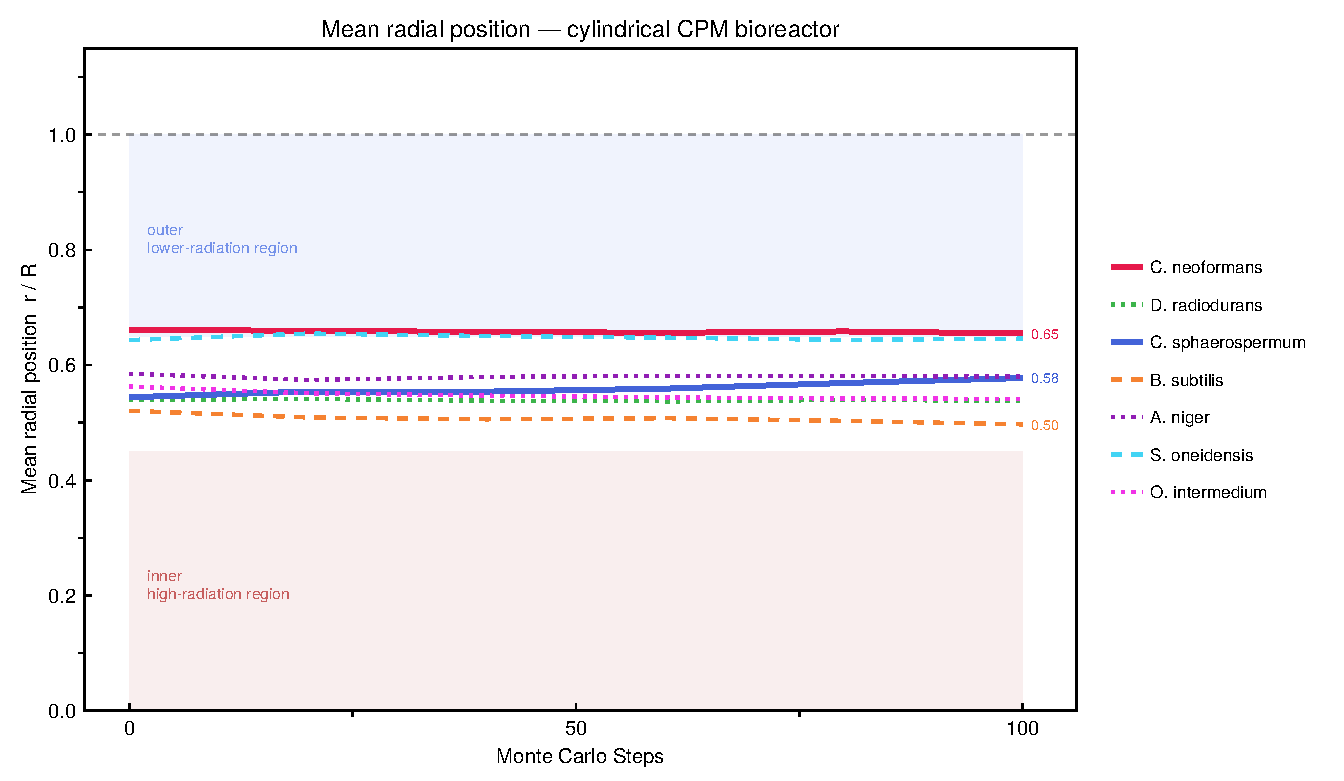
\includegraphics[width=0.85\linewidth]{fig1_radial_stratification}
\caption{Radial stratification of seven species over 100 Monte Carlo Steps in the cylindrical
CPM bioreactor.  Solid lines: radiotropic species (\textit{C.~neoformans}, \textit{C.~sphaerospermum}).
Dashed lines: remaining species.  Dashed horizontal line marks the cylinder wall ($r = R$).
The field is maximal on the axis, so the core is the high-dose region and the wall is the
low-dose one.  Over this single seed the radiotropic species end further out and
\textit{B.~subtilis} further in --- the direction opposite to the one their $\beta_{s,\mathrm{ion}}$
signs implement, and within about 1.5 standard errors of the uniform-seeding null at $n = 6$
parcels.  Whatever displacement the acceptance rule can produce comes from
$\Delta H_{\mathrm{mel}}$ and not from $\Delta H_{\mathrm{rad}}$
(Table~\ref{tab:term_magnitudes}).}
\label{fig:radial}
\end{figure}

\begin{figure}[htbp]
\centering
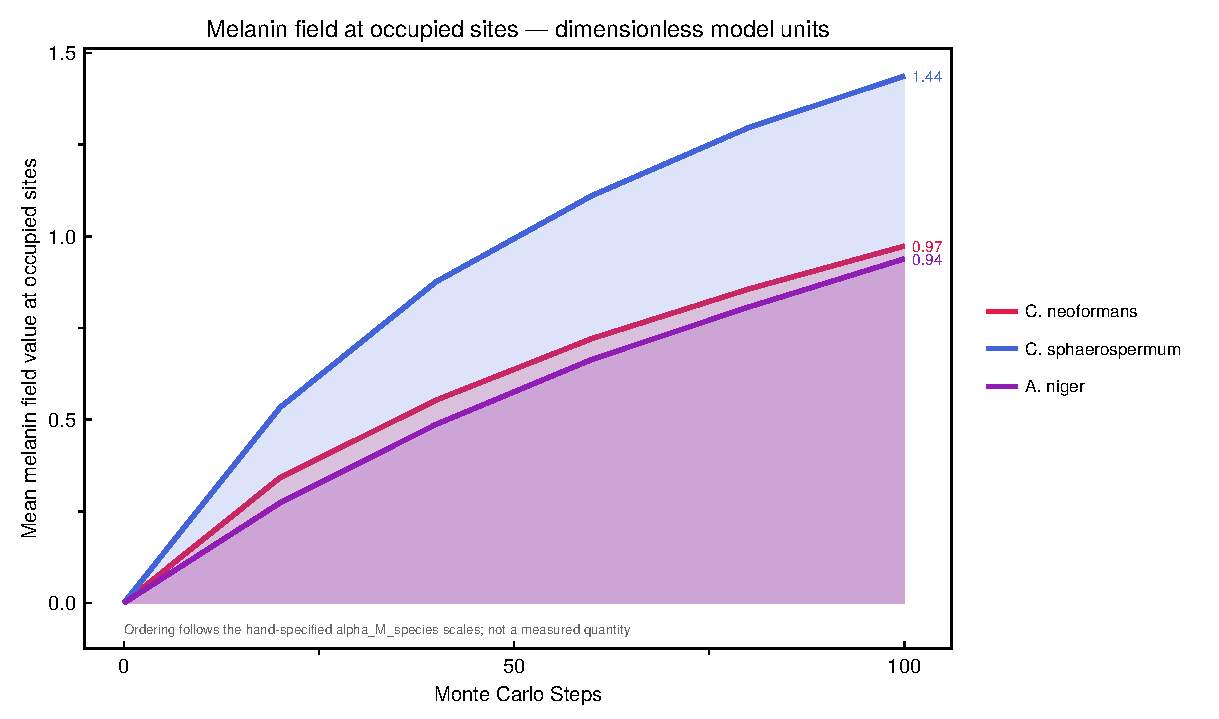
\includegraphics[width=0.78\linewidth]{fig2_melanin_accumulation}
\caption{Melanin field accumulation at occupied lattice sites for the three melanin-producing
species over 100~MCS.  Field values are dimensionless model units.
\textit{C.~sphaerospermum} (blue) accumulates most rapidly, following its highest $\alpha_M$
(Table~\ref{tab:params}); its radial position works against it rather than for it.
\textit{A.~niger} (purple) and \textit{C.~neoformans} (red) accumulate at intermediate rates.}
\label{fig:melanin}
\end{figure}

\subsection{Radiodialysis: Contaminant Transport Under a Time-Varying Wall Permeability}

\paragraph{Every number in this subsection is dimensionless.}
The coupled run has two clocks --- the CPM's Monte Carlo Step count and the transport solver's
seconds --- with no declared conversion between them: \texttt{seconds\_per\_mcs} ships as
\texttt{NaN} and the dose accrual routine raises rather than substitute a default. The dose rate
driving Eqs.~\ref{eq:membrane_damage}--\ref{eq:peff} in the coupled Julia port is a hard-coded
placeholder $\dot{D} = 1.0$, never derived from the radiation field, and the radial coordinate fed
to the solver is $N/2 = 20$ lattice units placed in a slot whose operator expects cm. An earlier
draft reported this run as ``50~Gy cumulative dose'' with a permeability rising from $P_0 = 0.01$ to
$0.027$~cm\,s$^{-1}$. Both are withdrawn: there is no gray here, and the cm\,s$^{-1}$ figure was
the Nafion-117 literature prior $P_0$ multiplied by the dimensionless ratio below. A literature
prior rescaled by a model output is not a calibration.

Over 100~MCS the membrane integrity variable falls from $m = 1.0$ to $m = 0.779$ and the
permeability ratio reaches $P_{\mathrm{eff}}/P_0 = e \approx 2.72$ (Figure~\ref{fig:membrane}).
The decay follows Eq.~\ref{eq:membrane_damage} exactly. The ratio is exactly $e$ by construction,
because $\alpha_P\,\dot{D}\,\Delta t_{rd}\,n_{\mathrm{MCS}} = 1$ for the four hand-set constants
shipped; it is a closed-form consequence of the parameter choice and not a measurement of anything.
The functional form of Eq.~\ref{eq:peff} is the one established for Nafion membranes under ionising
flux \cite{lara2023}, and that provenance is why it was chosen, not evidence that this run
reproduces it.

\paragraph{What the transport solution does show.}
The PDE system is correctly derived and is solved twice independently --- \texttt{deSolve}'s LSODA
in R and a substepped forward-Euler port in Julia --- with the two implementations in agreement.
That much is a genuine numerical result, and permeability as an evolving field driven by cumulative
dose, rather than as a fixed material property, is the mechanism worth taking from this work.
At the final step the wall value is $c(R,t) = 0.87\,c_{\mathrm{ext}}$ and the interior node mean is
$c_{\mathrm{mean}}/c_{\mathrm{ext}} = 0.024$ (Figure~\ref{fig:contaminant}).

\paragraph{Three readings those two numbers do not support.}
First, the low interior value measures \emph{non-penetration, not removal}: $c(t = 0) \equiv 0$
everywhere inside, so the interior never held contaminant that could be depleted, and an earlier
draft's ``the contaminant front is consumed within a thin annular shell'' asserts a spatial
structure the model cannot produce. The radial biomass profile is collapsed by an unweighted
\texttt{mean()} before it reaches the solver, so the uptake sink is spatially \emph{uniform}:
there is no annular shell in this discretisation. Second, $c_{\mathrm{mean}}$ is an unweighted mean
over radial nodes rather than a volume-weighted one, which under-weights the outer, contaminant-rich
annulus of a cylinder. Third, $c(R,t)$ is dominated by the imposed Robin condition, so it reads the
boundary rather than transport through the biofilm. The rate constants
$k_{\mathrm{ads}}$ and $k_{\mathrm{red}}$ carry cm$^3$\,g$^{-1}$\,s$^{-1}$ in the R model, but in
the coupled Julia port they multiply site-occupancy fractions rather than densities in
g\,cm$^{-3}$, and $X_{\mathrm{red}}$ counts one species' sites over \emph{all} interior sites, so
it is neither a biomass fraction nor a reducer fraction. The project's material gate records this
path as \texttt{RADIODIALYSIS: BLOCKED} --- blocked by a units error in the model, not by missing
data.

\paragraph{The self-regulating loop is a design hypothesis, not a result.}
An earlier draft opened this subsection by reporting ``a self-reinforcing remediation loop driven by
the radiation field itself''. No such loop runs. $m$ decays and $P_{\mathrm{eff}}$ grows as
independent open-loop functions of time and neither reads the other; $P_{\mathrm{eff}}$ is a
function of $t$ alone; and because the biomass profile is averaged to a scalar, where a species sits
cannot influence uptake. \textit{S.~oneidensis} does finish this run at mean $r = 12.9$, near the
contaminant entry zone, but that is subject to the same seeding null as the rest of
Section~\ref{sec:cpm_results} and, more decisively, it cannot matter to the transport result
because the solver never sees a radial biomass profile. The co-localisation claim is withdrawn.

\begin{figure}[htbp]
\centering
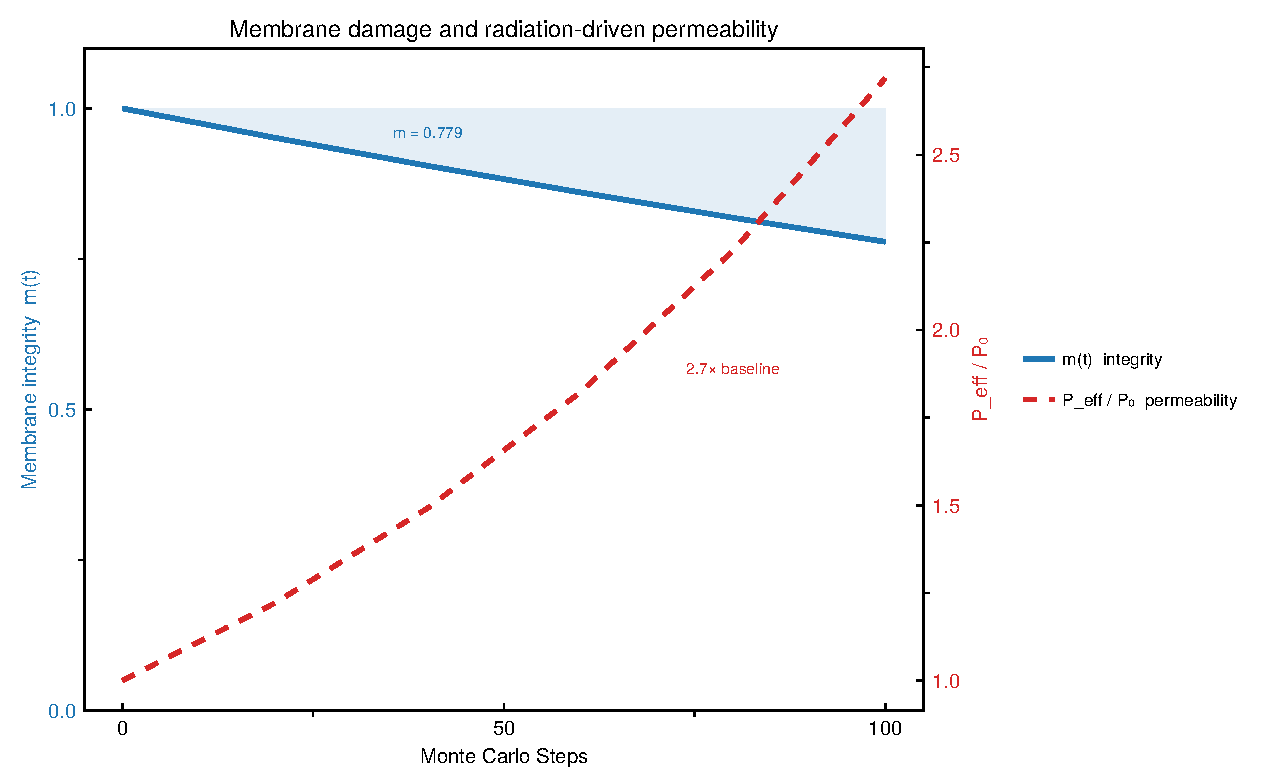
\includegraphics[width=0.85\linewidth]{fig3_membrane_transport}
\caption{Membrane integrity $m(t)$ (solid, left axis) and normalised effective permeability
$P_{\mathrm{eff}}(t)/P_0$ (dashed, right axis) over 100~MCS.  $m(t)$ decays exponentially
per Eq.~\ref{eq:membrane_damage}; $P_{\mathrm{eff}}/P_0$ rises per Eq.~\ref{eq:peff}.  Both axes
are dimensionless and the horizontal axis is MCS, not seconds: no MCS-to-second conversion exists,
so no cumulative dose in gray can be assigned to this run.  At MCS~100, $m = 0.779$ and
$P_{\mathrm{eff}}/P_0 = e \approx 2.72$, the latter exactly by construction from four hand-set
constants.}
\label{fig:membrane}
\end{figure}

\begin{figure}[htbp]
\centering
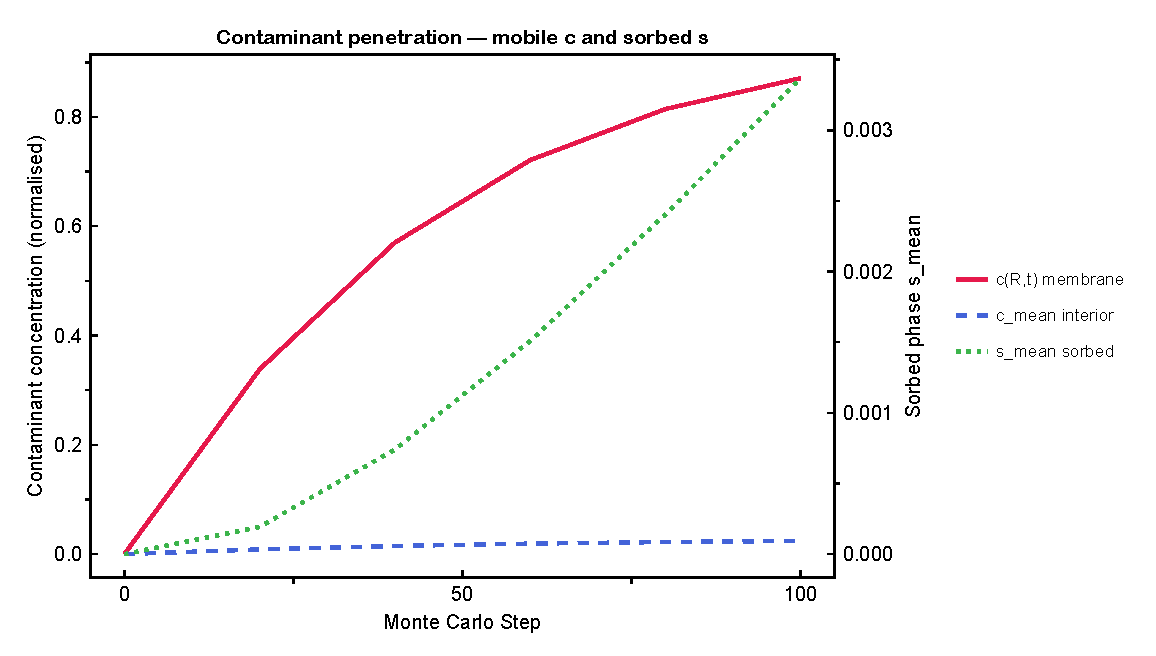
\includegraphics[width=0.85\linewidth]{fig4_contaminant_penetration}
\caption{Contaminant penetration over 100~MCS.  Red solid: $c(R,t)$, mobile concentration at
the membrane face.  Blue dashed: $c_{\mathrm{mean}}$, spatial average over the interior.
Green dotted (right axis): $s_{\mathrm{mean}}$, sorbed/immobilised phase.  All quantities are
dimensionless ratios to $c_{\mathrm{ext}}$ and the horizontal axis is MCS.  The near-zero interior
value measures non-penetration and not removal, since $c(t=0) \equiv 0$ everywhere inside; the
uptake sink is spatially uniform, so the figure shows no annular structure; and
$c_{\mathrm{mean}}$ is an unweighted mean over radial nodes rather than a volume-weighted one.}
\label{fig:contaminant}
\end{figure}

% ---- 7. Discussion -------------------------------------------
\section{Discussion}

\subsection{The Hamiltonian Framework Versus Classical Biofilm Models}

The phase-locked Hamiltonian framework differs fundamentally from prior reaction-diffusion
biofilm models in its treatment of inter-species interactions and energy conservation.
Classical models following the Wanner-Gujer tradition \cite{wanner1986} describe biofilm
dynamics through coupled PDEs governing substrate consumption and biomass growth, with species
interactions mediated exclusively through competition for shared substrates. Our Hamiltonian
$H(p,q)$ is written to conserve total system energy across kinetic, potential and interaction
terms. That is a property of the formalism in Eq.~\ref{eq:hamiltonian} and not of any program
reported here: no simulation performs symplectic integration \cite{hairer2006}, none carries a
momentum state, and the CPM's $H$ is a Metropolis acceptance functional in arbitrary units,
dissipated toward a minimum rather than conserved (Section~3.4). The same caution applies to the
fluctuation-dissipation argument: the stochastic layer is intended to add thermal and demographic
noise while preserving the Hamiltonian structure, and demonstrating that it does would require the
integrator that does not yet exist. The structure is intended to capture phenomena that ODE/PDE
models miss --- synchronised oscillations through phase-locking, and energy-conserving transitions
between fitness states --- though the phase-locking component remains specified rather than
exercised (Section~6.4).

An earlier draft claimed a further distinction: ``between radiation as a damaging perturbation
versus radiation as an energy source positively coupled to the Hamiltonian''. That is withdrawn.
The CPM Hamiltonian is a Metropolis acceptance functional in arbitrary units, not an energy budget,
and a negative $\beta_{\mathrm{ion}}$ in it is a spatial preference, not a metabolic gain: the
model creates no biomass for such a gain to act on. What the sign of $\beta_{\mathrm{ion}}$ buys is
a directional response, which is a real and useful thing for a spatial model to express, and it
should be claimed as that and not as energy transduction.

\subsection{Biological Interpretation of \textit{C.\ neoformans} and \textit{D.\ radiodurans} Dynamics}

The contrast between \textit{C.\ neoformans} and \textit{D.\ radiodurans} in this framework
illuminates a distinction that the loose vocabulary of the field routinely collapses, and getting
it right constrains what the model may be said to show.

\textit{D.\ radiodurans} is radioresistant. That is a survival phenotype, measured as $D_{10}$, and
it is the best-evidenced radiation phenotype among the seven species here, resting on
Mn$^{2+}$-dependent proteome shielding and efficient double-strand break repair
\cite{daly2010,slade2011}. \textit{C.\ neoformans} is melanized, and melanin measurably alters
several radiation responses; whether it enhances growth under a photon field is contested
(Section~2.1), and whether it protects survival under sparsely-ionizing photons is not established
even in the one study that reports melanin protection under deuterons, where the same species'
X-ray result is hedged \cite{audit2026}.

Neither phenotype is what this model computes. The simulations reported here have no death term, so
they cannot express radioresistance, and no growth term, so they cannot express radiotrophy; both
are structurally absent rather than weakly supported, and no quantity of additional data changes
that without a model revision. An earlier draft stated that \textit{C.\ neoformans} ``increases its
fitness monotonically with radiation intensity'', that $\gamma_s$ ``converts absorbed dose into
fitness gain via the melanin-mediated electron-transfer pathway'', and that the model ``correctly
predicts that \textit{C.\ neoformans} outcompetes \textit{D.\ radiodurans} in moderately irradiated
environments''. All three are withdrawn: the first two describe Eq.~\ref{eq:psde} as written rather
than any simulation performed, and the third describes a competitive outcome that nothing here
computes.

What the model does express is that the two species occupy different positions in the dose field
for different parameterised reasons, and it separates the mechanisms cleanly enough that the
distinction is visible in the spatial output. That is a modest claim and it is defensible. The
electron-transfer literature \cite{turick2011,casadevall2017} motivates the melanin term; it does
not calibrate it.

\subsection{Implications for Nuclear Bioremediation}

This subsection is a design hypothesis. It is stated as one because no simulation reported here
computes any part of it, and an earlier draft stated it as a model prediction.

The hypothesis: in a Th-contaminated environment, \textit{S.\ oneidensis}, with its capacity for
extracellular electron transfer to metal oxides \cite{heidelberg2002,veeramani2011}, reduces
soluble actinide species and immobilises them as insoluble precipitates, but its extreme
radiosensitivity ($D_{10} \approx 0.07$~kGy) limits viability in high-dose zones;
\textit{O.\ intermedium} AM7, with its thorium-tolerant EPS production \cite{shukla2020},
establishes a matrix that attenuates local dose sufficiently to permit \textit{S.\ oneidensis}
colonisation further in. That would be a synergy worth engineering for.

Nothing here tests it, and three specific gaps say why. \textbf{No model in this work attenuates
radiation by biomass.} The gamma field is initialised once from Beer--Lambert geometry
(Eq.~\ref{eq:gamma_field}) and never updated; biomass occupancy is not a term in it and no feedback
runs from the community back to the field, so a protective matrix cannot exist in these simulations
even in principle. \textbf{The dose-response that would make attenuation matter is absent.} There
is no death term anywhere (Section~\ref{sec:limitations}), so a species cannot be excluded from a
zone by dose, and a lower local dose cannot permit a colonisation that a higher one prevented.
\textbf{And \textit{O.\ intermedium} AM7 is not in the Langevin models at all} --- it appears in
the Julia CPM registry only, so the earlier draft's ``emergent from the Langevin dynamics''
attribution named a simulation that never instantiated the organism. Adding a dose-dependent
survival term and a two-way radiation field are the two model changes that would make this
hypothesis testable; both are listed in Section~\ref{sec:limitations}. The potential for
engineering \textit{D.\ radiodurans} strains for combined radioresistance and metal reduction
\cite{brim2000} is likewise cited as literature, not as an output.

A second design hypothesis follows from the membrane model
(Section~\ref{sec:radiodialysis}), and it is the more interesting of the two. In a conventional
passive membrane reactor, contaminant ingress is fixed by the membrane's baseline permeability
$P_0$. Treating permeability instead as a field driven by cumulative dose
(Eq.~\ref{eq:peff}) proposes a loop: higher ambient radiation $\to$ faster membrane
permeabilisation $\to$ greater contaminant ingress $\to$ greater substrate availability for
metal-reducing bacteria, with the contamination source supplying both the chemical substrate and
the physical driver, and requiring no external energy input.

\textbf{Every arrow in that chain is currently open, and the code says so.}
$m$ and $P_{\mathrm{eff}}$ are independent laws in the implementation and neither reads the other;
$P_{\mathrm{eff}}$ is a function of $t$ alone, so it is open-loop even with respect to the dose it
is supposed to integrate; the radial biomass profile is averaged to a scalar before reaching the
transport solver, so where a species sits cannot influence uptake; and no feedback runs from biology
to the radiation field or to the membrane anywhere in this work. The project retains an explicit
stop condition on exactly this point: no transported dose enters the radiodialysis model until the
constitutive choice between the decaying $m$ and the growing $P_{\mathrm{eff}}$ is selected, because
wiring the loop before that choice would hard-code an unexamined assumption about how damage maps to
permeability. This is therefore a hypothesis the framework was built to make testable, and it is not
yet tested. Reactor design implications --- prioritising membrane materials with intermediate
$\alpha_P$ (Eq.~\ref{eq:peff}), high enough to self-tune under operational dose rates but low
enough to prevent catastrophic failure \cite{fox2009,lara2023} --- follow from the proposal and not
from any result reported here.

\subsection{Mechanical Properties and Radiation Survival}

\textbf{Both components of Section~3.10 are specification.} A case-insensitive search of every
source file in this project returns no FENE potential and no Kelvin-Voigt element; neither
Eq.~\ref{eq:fene} nor Eq.~\ref{eq:kelvinvoigt} is evaluated by any simulation, and no stress,
strain or modulus is a state variable anywhere. What follows is the motivation for carrying them in
the formalism, not a description of model behaviour.

Biofilm EPS matrices exhibit viscoelastic behaviour that mediates mechanical stress transmission,
nutrient diffusion resistance and protection from external perturbations --- a dimension of biofilm
physics largely absent from ecological radiation models. A FENE potential would supply the finite
extensibility that prevents unphysical deformation under radiation-induced swelling or thermal
expansion; a Kelvin-Voigt element would capture stress relaxation on timescales relevant to biofilm
restructuring. The mechanism this would let the framework express --- species with higher EPS
production rates (\textit{O.\ intermedium} AM7, \textit{B.\ subtilis}) generating stiffer local
environments and so protected microniches for radiosensitive community members --- is a hypothesis
about a model that has not been built. An earlier draft asserted it as a property of this one.

\subsection{Limitations and Future Directions}
\label{sec:limitations}

\paragraph{What the model structurally cannot express.}
There is no birth and no death anywhere in the four simulations. Radiotrophy requires growth and
radioresistance requires death, so neither is representable here at any parameter value: they are
structurally absent, not weakly supported, and the distinction matters because the remedy is a
model revision rather than a measurement. Adding a dose-dependent survival term is the single
change that would let this framework consume the excellent $D_{10}$ literature as calibration data
rather than as motivation for a tropism coefficient. Directed hyphal elongation --- the one
measured radiotropism candidate in the literature --- is likewise unrepresentable while agents are
isotropic biomass parcels with no elongation or connectivity term.

\paragraph{Identifiability.}
Only the product of the melanin production rate $\alpha_M$ and the melanin coupling constant
reaches the CPM dynamics (Section~\ref{sec:cpm_results}), so the two cannot be fitted separately
however much data arrives. This is a structural limit and it should be stated wherever either
parameter is quoted.

\paragraph{Nothing here is calibrated.}
No value in Table~\ref{tab:params} is fitted to data from this system; the lattice pitch, the
biomass density, the seconds-per-Monte-Carlo-Step conversion and the Hamiltonian and melanin
normalisations are all unpopulated. Consequently the CPM's spatial and temporal outputs are
dimensionless model quantities and are reported as such. No public dataset can currently close this
gap: no source pairs an exact modelled species with both a calibrated 3-D biomass field and a
characterised radiation exposure, and none pairs a calibrated hydrated volume with wet mass, dry
mass and matched blanks for any organism \cite{audit2026}. Those measurements must be acquired, not
retrieved.

\paragraph{Physical simplifications.}
The radiation field is treated as radially symmetric with exponential attenuation
(Eq.~\ref{eq:gamma_field}), whereas actual environments at Chernobyl and Hanford exhibit complex
three-dimensional dose distributions governed by heterogeneous source geometries and shielding
materials. The UV oscillatory term (Eq.~\ref{eq:uv_field}) assumes a purely sinusoidal diurnal
cycle, neglecting atmospheric absorption spectra and seasonal variation. The model does not
incorporate horizontal gene transfer, which is known to spread radiation resistance determinants
among biofilm community members.

\paragraph{Future directions.}
Implement and test the phase-locking kernel $H_{\mathrm{kNN}}$ (Eq.~\ref{eq:knn}), which is
currently specified but unexercised. Add growth and death so that the framework can represent
radiotrophy and radioresistance rather than only radiotropism. Run the sensitivity analysis this
paper does not have --- noting that a sweep over $\beta_{s,\mathrm{ion}}$ alone would miss the
mechanism entirely (Section~\ref{sec:cpm_results}). Couple the model to measured dose-rate maps
from contaminated facilities. Incorporate spatially resolved nutrient transport by Darcy flow
through the EPS matrix. And acquire the paired experiment the evidence audit specifies: on one
system under one growth condition, replicate-level wet and dry mass with matched blanks, a
hydrated volume on a whole-biofilm-envelope basis, closed elemental composition on a wet-bulk
basis, a calibrated 3-D stack of the same specimen, and a characterised dose field with a measured
gradient.

% ---- 8. Conclusion -------------------------------------------
\section{Conclusion}

This work introduces a Hamiltonian-Langevin framework for modelling radiotropic spatial fitness in
multispecies biofilm communities exposed to ionising radiation. The PSDE fitness equation
(Eq.~\ref{eq:psde}) couples radiation-dependent terms, melanin reaction-diffusion, stochastic
demographic noise, and viscoelastic biofilm mechanics into a single formalism, and the Cellular
Potts implementation resolves it at the level of biomass parcels on a cylindrical lattice.

The central result of this revision is not the radial pattern but an accounting of the acceptance
rule that could produce one. Within the radiation-derived pathway the melanin term dominates the
per-species $\beta_{s,\mathrm{ion}}$ that Table~\ref{tab:params} tabulates and that the entire sign
convention is written around: at the shipped constants the two differ in Metropolis acceptance bias
by four orders of magnitude (Table~\ref{tab:term_magnitudes}), 15.5\% against one part in $10^5$.
Radiation therefore reaches the dynamics indirectly, through melanin production, and only the
product of the two melanin coefficients is identifiable at all. That finding is arithmetic on
shipped constants and does not depend on any run.

The radial pattern itself is reported as a diagnostic and not as an established result. On one seed
with six parcels per species the melanized fungi (\textit{C.\ neoformans},
\textit{C.\ sphaerospermum}) finish further from the axis than \textit{B.\ subtilis} --- the
direction opposite to the one their negative $\beta_{s,\mathrm{ion}}$ implements, since the field is
maximal on the axis and the core is the high-dose region --- and the gap is about 1.5 standard
errors of the uniform-seeding null (Section~\ref{sec:cpm_results}). Replicate seeds against that
null are the cheapest outstanding experiment in this work.

One further qualification travels with all of it: the phenotype expressed is radiotropism alone.
With no growth and no death in the model, radiotrophy and radioresistance are structurally absent,
and the strong published $D_{10}$ evidence that anchors the coefficient magnitudes is
radioresistance evidence spent on a tropism term.

Radiotrophy, moreover, is not established for any of the seven species modelled
(Section~\ref{sec:radiotrophy_status}); radioresistance is. Nothing in this framework is calibrated
against a measurement of the system it models, and no public dataset can currently supply that
calibration. The natural next steps are therefore two, and they are separable: add growth and
survival so the framework can consume the radiobiology literature as data rather than as
motivation, and acquire the paired morphology-plus-dosimetry experiment that would let its spatial
outputs be reported in physical units.

% ---- References ---------------------------------------------
\begin{thebibliography}{38}

\bibitem{zhdanova2000}
Zhdanova, N.N., Zakharchenko, V.A., Vember, V.V., Nakonechnaya, L.T. (2000).
Fungi from Chernobyl: mycobiota of the inner regions of the containment structures of the
damaged nuclear reactor.
\textit{Mycological Research}, 104(12), 1421--1426.
\url{https://doi.org/10.1017/S0953756200002756}

\bibitem{dadachova2007}
Dadachova, E., Bryan, R.A., Huang, X., Moadel, T., Schweitzer, A.D., Aisen, P.,
Nosanchuk, J.D., Casadevall, A. (2007).
Ionizing radiation changes the electronic properties of melanin and enhances the growth of
melanized fungi.
\textit{PLoS ONE}, 2(5), e457.
\url{https://doi.org/10.1371/journal.pone.0000457}

\bibitem{dadachova2008}
Dadachova, E., Casadevall, A. (2008).
Ionizing radiation: how fungi cope, adapt, and exploit with the help of melanin.
\textit{Current Opinion in Microbiology}, 11(6), 525--531.
\url{https://doi.org/10.1016/j.mib.2008.09.013}

\bibitem{shunk2022}
Shunk, G.K., Gomez, X.R., Kern, C., Averesch, N.J.H. (2022).
Cultivation of the dematiaceous fungus \textit{Cladosporium sphaerospermum} aboard the
International Space Station and effects of ionizing radiation.
\textit{Frontiers in Microbiology}, 13, 877625.
\url{https://doi.org/10.3389/fmicb.2022.877625}

\bibitem{slade2011}
Slade, D., Radman, M. (2011).
Oxidative stress resistance in \textit{Deinococcus radiodurans}.
\textit{Microbiology and Molecular Biology Reviews}, 75(1), 133--191.
\url{https://doi.org/10.1128/MMBR.00015-10}

\bibitem{daly2009}
Daly, M.J. (2009).
A new perspective on radiation resistance based on \textit{Deinococcus radiodurans}.
\textit{Nature Reviews Microbiology}, 7(3), 237--245.
\url{https://doi.org/10.1038/nrmicro2073}

\bibitem{daly2010}
Daly, M.J., et al. (2010).
Small-molecule antioxidant proteome-shields in \textit{Deinococcus radiodurans}.
\textit{PLoS ONE}, 5(9), e12570.
\url{https://doi.org/10.1371/journal.pone.0012570}

\bibitem{wanner1986}
Wanner, O., Gujer, W. (1986).
A multispecies biofilm model.
\textit{Biotechnology and Bioengineering}, 28(3), 314--328.
\url{https://doi.org/10.1002/bit.260280304}

\bibitem{xavier2005}
Xavier, J.B., Picioreanu, C., van Loosdrecht, M.C.M. (2005).
A framework for multidimensional modelling of activity and structure of multispecies biofilms.
\textit{Environmental Microbiology}, 7(8), 1085--1103.
\url{https://doi.org/10.1111/j.1462-2920.2005.00787.x}

\bibitem{lardon2011}
Lardon, L.A., et al. (2011).
iDynoMiCS: next-generation individual-based modelling of biofilms.
\textit{Environmental Microbiology}, 13(9), 2416--2434.
\url{https://doi.org/10.1111/j.1462-2920.2011.02414.x}

\bibitem{sonner2015}
Sonner, S., Efendiev, M.A., Eberl, H.J. (2015).
On the well-posedness of a mathematical model of quorum-sensing in patchy biofilm communities.
\textit{Mathematical Methods in the Applied Sciences}, 38(3), 3037--3042.
\url{https://doi.org/10.1002/mma.3237}

\bibitem{diele2015}
Diele, F., Marangi, C., Ragni, S. (2015).
Geometric numerical integration in ecological modelling.
\textit{Mathematics and Computers in Simulation}, 110, 40--52.
\url{https://doi.org/10.1016/j.matcom.2014.02.006}

\bibitem{kuramoto1984}
Kuramoto, Y. (1984).
\textit{Chemical Oscillations, Waves, and Turbulence}.
Springer-Verlag, Berlin.
\url{https://doi.org/10.1007/978-3-642-69689-3}

\bibitem{acebron2005}
Aceb\'r\'on, J.A., Bonilla, L.L., P\'erez Vicente, C.J., Ritort, F., Spigler, R. (2005).
The Kuramoto model: a simple paradigm for synchronization phenomena.
\textit{Reviews of Modern Physics}, 77(1), 137--185.
\url{https://doi.org/10.1103/RevModPhys.77.137}

\bibitem{campillo2017}
Campillo, F., Joannides, M., Larramendy-Valverde, I. (2017).
Stochastic analysis of a full system of two competing populations in a chemostat.
\textit{Chemical Engineering Science}, 175, 424--440.
\url{https://doi.org/10.1016/j.ces.2017.10.052}

\bibitem{heidelberg2002}
Heidelberg, J.F., et al. (2002).
Genome sequence of the dissimilatory metal ion-reducing bacterium
\textit{Shewanella oneidensis}.
\textit{Nature Biotechnology}, 20(11), 1118--1123.
\url{https://doi.org/10.1038/nbt749}

\bibitem{veeramani2011}
Veeramani, H., et al. (2011).
Products of abiotic U(VI) reduction by biogenic magnetite and vivianite.
\textit{Geochimica et Cosmochimica Acta}, 75(9), 2512--2528.
\url{https://doi.org/10.1016/j.gca.2011.02.024}

\bibitem{shukla2020}
Shukla, A., Parmar, P., Goswami, D., Patel, B., Saraf, M. (2020).
Characterization of novel thorium tolerant \textit{Ochrobactrum intermedium} AM7.
\textit{Journal of Hazardous Materials}, 388, 122047.
\url{https://doi.org/10.1016/j.jhazmat.2020.122047}

\bibitem{wright1932}
Wright, S. (1932).
The roles of mutation, inbreeding, crossbreeding and selection in evolution.
\textit{Proceedings of the Sixth International Congress of Genetics}, 1, 356--366.

\bibitem{kauffman1989}
Kauffman, S.A., Weinberger, E.D. (1989).
The NK model of rugged fitness landscapes.
\textit{Journal of Theoretical Biology}, 141(2), 211--245.
\url{https://doi.org/10.1016/S0022-5193(89)80019-0}

\bibitem{berg1993}
Berg, H.C. (1993).
\textit{Random Walks in Biology}.
Princeton University Press.

\bibitem{guttenplan2013}
Guttenplan, S.B., Shaw, S., Kearns, D.B. (2013).
The cell biology of peritrichous flagella in \textit{Bacillus subtilis}.
\textit{Molecular Microbiology}, 87(1), 211--229.
\url{https://doi.org/10.1111/mmi.12103}

\bibitem{nicholson2000}
Nicholson, W.L., et al. (2000).
Resistance of \textit{Bacillus} endospores to extreme terrestrial and extraterrestrial
environments.
\textit{Microbiology and Molecular Biology Reviews}, 64(3), 548--572.
\url{https://doi.org/10.1128/MMBR.64.3.548-572.2000}

\bibitem{turick2011}
Turick, C.E., et al. (2011).
Gamma radiation interacts with melanin to alter its oxidation-reduction potential and
results in electric current production.
\textit{Bioelectrochemistry}, 82(1), 69--73.
\url{https://doi.org/10.1016/j.bioelechem.2011.04.009}

\bibitem{robertson2012}
Robertson, K.L., et al. (2012).
Adaptation of the black yeast \textit{Wangiella dermatitidis} to ionizing radiation.
\textit{PLoS ONE}, 7(11), e48674.
\url{https://doi.org/10.1371/journal.pone.0048674}

\bibitem{malo2018}
Malo, M.E., et al. (2018).
Morphological changes in melanized and non-melanized \textit{Cryptococcus neoformans} cells
post exposure to ionizing radiation.
\textit{Fungal Biology}, 122(6), 449--456.
\url{https://doi.org/10.1016/j.funbio.2017.08.012}

\bibitem{newsome2014}
Newsome, L., Morris, K., Lloyd, J.R. (2014).
The biogeochemistry and bioremediation of uranium and other priority radionuclides.
\textit{Chemical Geology}, 363, 164--184.
\url{https://doi.org/10.1016/j.chemgeo.2013.10.034}

\bibitem{brim2000}
Brim, H., et al. (2000).
Engineering \textit{Deinococcus radiodurans} for metal remediation in radioactive mixed
waste environments.
\textit{Nature Biotechnology}, 18(1), 85--90.
\url{https://doi.org/10.1038/71986}

\bibitem{kazy2009}
Kazy, S.K., D'Souza, S.F., Sar, P. (2009).
Uranium and thorium sequestration by a \textit{Pseudomonas} sp.
\textit{Journal of Hazardous Materials}, 163(1), 65--72.
\url{https://doi.org/10.1016/j.jhazmat.2008.06.076}

\bibitem{blasius1999}
Blasius, B., Huppert, A., Stone, L. (1999).
Complex dynamics and phase synchronization in spatially extended ecological systems.
\textit{Nature}, 399, 354--359.
\url{https://doi.org/10.1038/20676}

\bibitem{alpkvist2007}
Alpkvist, E., Klapper, I. (2007).
A multidimensional multispecies continuum model for heterogeneous biofilm development.
\textit{Bulletin of Mathematical Biology}, 69(2), 765--789.
\url{https://doi.org/10.1007/s11538-006-9168-7}

\bibitem{eberl2001}
Eberl, H.J., Parker, D.F., van Loosdrecht, M.C.M. (2001).
A new deterministic spatio-temporal continuum model for biofilm development.
\textit{Journal of Theoretical Medicine}, 3(3), 161--175.
\url{https://doi.org/10.1080/10273660108833072}

\bibitem{hairer2006}
Hairer, E., Lubich, C., Wanner, G. (2006).
\textit{Geometric Numerical Integration}, 2nd ed.
Springer-Verlag.
\url{https://doi.org/10.1007/3-540-30666-8}

\bibitem{eisenman2012}
Eisenman, H.C., Casadevall, A. (2012).
Synthesis and assembly of fungal melanin.
\textit{Applied Microbiology and Biotechnology}, 93(3), 931--940.
\url{https://doi.org/10.1007/s00253-011-3777-2}

\bibitem{lloyd2005}
Lloyd, J.R., Renshaw, J.C. (2005).
Bioremediation of radioactive waste.
\textit{Current Opinion in Biotechnology}, 16(3), 254--260.
\url{https://doi.org/10.1016/j.copbio.2005.04.012}

\bibitem{khajo2011}
Khajo, A., et al. (2011).
Protection of melanized \textit{Cryptococcus neoformans} from lethal dose gamma irradiation.
\textit{PLoS ONE}, 6(9), e25092.
\url{https://doi.org/10.1371/journal.pone.0025092}

\bibitem{battista1997}
Battista, J.R. (1997).
Against all odds: the survival strategies of \textit{Deinococcus radiodurans}.
\textit{Annual Review of Microbiology}, 51, 203--224.
\url{https://doi.org/10.1146/annurev.micro.51.1.203}

\bibitem{casadevall2017}
Casadevall, A., et al. (2017).
Melanin, radiation, and energy transduction in fungi.
\textit{Microbiology Spectrum}, 5(2), FUNK-0037-2016.
\url{https://doi.org/10.1128/microbiolspec.FUNK-0037-2016}

\bibitem{graner1992}
Graner, F., Glazier, J.A. (1992).
Simulation of biological cell sorting using a two-dimensional extended Potts model.
\textit{Physical Review Letters}, 69(13), 2013--2016.
\url{https://doi.org/10.1103/PhysRevLett.69.2013}

\bibitem{fox2009}
Fox, E.B., et al. (2009).
Radiation effects on Nafion$^{\circledR}$ membrane properties.
\textit{Savannah River National Laboratory Technical Report}, SRNL-STI-2009-00053.

\bibitem{lara2023}
Lara, D., et al. (2023).
Ionizing radiation effects on proton exchange membrane permeability and selectivity.
\textit{Membranes}, 13(4), 412.
\url{https://doi.org/10.3390/membranes13040412}

\bibitem{renslow2017}
Renslow, R.S., et al. (2017).
Modeling biofilm-mediated uranium immobilization in porous media.
\textit{Water Research}, 109, 120--130.
\url{https://doi.org/10.1016/j.watres.2016.11.038}

\bibitem{aydogan2022}
Aydogan Gokturk, P., Sujanani, R., Qian, J., Wang, L., Freyman, J.L., Bhatt, A.D.,
Freeman, B.D., Bhave, R., Boudouris, B.W., Phillip, W.A. (2022).
Donnan dialysis of monovalent ions across a cation exchange membrane.
\textit{Nature Communications}, 13, 5258.
\url{https://doi.org/10.1038/s41467-022-32930-9}

\bibitem{soetaert2010}
Soetaert, K., Petzoldt, T., Setzer, R.W. (2010).
Solving differential equations in R: package deSolve.
\textit{Journal of Statistical Software}, 33(9), 1--25.
\url{https://doi.org/10.18637/jss.v033.i09}

\bibitem{cortesao2020}
Cortes\~{a}o, M., et al. (2020).
Aspergillus niger spores are highly resistant to space radiation.
\textit{Frontiers in Microbiology}, 11, article 560.
(LD$_{90}$ values for N402 and the pigmentation-deficient $\Delta fwnA$ mutant MA93.1 under
X-ray, He-ion and Fe-ion exposure; open access, CC BY 4.0.)

\bibitem{walberg2015}
Walberg, K. (2015).
Assessment of the evidence for radiosynthesis in melanized fungi.
Undergraduate thesis, University of Wisconsin--La Crosse. \texttt{handle:1793/73406}.
(Licence not specified in the repository record. Contains no new measurement; the argument is a
closed energy budget plus a media-carbon confounder.)

\bibitem{audit2026}
Kinder, H., Faulkner, B. (2026).
Radiotrophic compatibility audit: public evidence for the radiation phenotypes of seven modelled
species. Project technical record, \texttt{docs/research/radiotrophic\_compatibility\_audit.md},
commits \texttt{904b9a4} and \texttt{a03bc32}, repository revision \texttt{5d1b777}.
(Eleven data repositories, the NCBI archives and Europe PMC searched at API level; every phenotype
label assigned from the endpoint actually measured; every unverified quantity recorded as
unverified. Four verdicts, quoted in Section~\ref{sec:radiotrophy_status}. This record populates no
parameter.)

\end{thebibliography}

\end{document}
